\documentclass[10pt]{article}
\usepackage{tmlr}

\input{math_commands.tex}
% Generated by tools/build_audit_latex_assets.py. Do not hand edit.
\newcommand{\CorpusTotal}{327}
\newcommand{\CanonicalWorkTotal}{325}
\newcommand{\OriginalCorpusTotal}{247}
\newcommand{\SupplementalCorpusTotal}{80}
\newcommand{\AuditedTotal}{304}
\newcommand{\AuditedWorkTotal}{302}
\newcommand{\DualReviewedTotal}{302}
\newcommand{\DualReviewedWorkTotal}{300}
\newcommand{\CodexOnlyWorkTotal}{2}
\newcommand{\BlockedTotal}{23}
\newcommand{\ImplementedTotal}{217}
\newcommand{\MedicalImplementedTotal}{192}
\newcommand{\NLevelZero}{38}
\newcommand{\NLevelOne}{74}
\newcommand{\NLevelTwo}{35}
\newcommand{\NLevelThree}{17}
\newcommand{\NLevelFour}{53}


\usepackage{hyperref}
\hypersetup{hidelinks}
\usepackage{url}
\usepackage{graphicx}
\usepackage{booktabs}
\usepackage{tabularx}
\usepackage{array}
\usepackage{tikz}
\usepackage{enumitem}
\usepackage{xcolor}
\usepackage{colortbl}
\usepackage{fontawesome5}
\usepackage{placeins}
\renewcommand{\topfraction}{0.92}
\renewcommand{\bottomfraction}{0.8}
\renewcommand{\textfraction}{0.07}
\renewcommand{\floatpagefraction}{0.7}
\setcounter{topnumber}{3}
\setcounter{totalnumber}{5}
\usetikzlibrary{arrows.meta,positioning,calc,decorations.pathmorphing,shadows.blur,fit,backgrounds}

\definecolor{mwmink}{HTML}{1A2A3A}
\definecolor{mwmblue}{HTML}{0072B2}
\definecolor{mwmteal}{HTML}{009E73}
\definecolor{mwmamber}{HTML}{E69F00}
\definecolor{mwmvermillion}{HTML}{D55E00}
\definecolor{mwmgray}{HTML}{6E7B8B}
\definecolor{mwmlight}{HTML}{DDE3E8}
\colorlet{mwmorange}{mwmamber}
\colorlet{mwmred}{mwmvermillion}
\colorlet{mwmgreen}{mwmteal}
\colorlet{mwmyellow}{mwmamber}
\tikzset{
  hand/.style={decorate, decoration={random steps, segment length=1.8mm, amplitude=0.4pt}},
  hbox/.style 2 args={hand, draw=#1, line width=1pt, rounded corners=2pt, fill=#2,
    blur shadow={shadow blur steps=4, shadow xshift=0.4pt, shadow yshift=-0.5pt}},
  harrow/.style={hand, -{Latex[length=2.0mm]}, line width=0.9pt},
  hdash/.style={hand, -{Latex[length=2.0mm]}, line width=0.8pt, densely dashed},
}
\newcommand{\cgood}{\textcolor{mwmteal}{\faCheck}\,}
\newcommand{\cpart}{\textcolor{mwmamber}{\faAdjust}\,}
\newcommand{\cgap}{\textcolor{mwmgray}{\faMinus}\,}
\newcommand{\mwmbar}[1]{\textcolor{mwmblue!72}{\rule{#1em}{1.05ex}}}

\title{Medical World Models: From Static Prediction to Clinically Valid Action-Aware Simulation}
\author{\name Anonymous Authors \email anonymous@example.com \\
      \addr Anonymous Institution}

\newcommand{\mwms}{medical world models}
\newcommand{\state}{state}
\newcommand{\action}{action}
\newcommand{\transition}{transition}
\newcommand{\outcome}{outcome}
\newcommand{\satotext}{state--action--transition--outcome}
\newenvironment{casebox}[1]{\par\smallskip\noindent\begin{minipage}{\linewidth}\hrule\vspace{0.55em}\textbf{Case study: #1}\par\smallskip\small}{\vspace{0.55em}\hrule\end{minipage}\par\smallskip}
\newcommand{\levelsummary}[3]{%
  \begin{center}
  \fcolorbox{mwmteal!75!black}{mwmteal!5}{%
    \begin{minipage}{0.94\linewidth}\small
    \textbf{Established.} #1\par\smallskip
    \textbf{Our assessment.} #2\par\smallskip
    \textbf{Next threshold.} #3
    \end{minipage}}
  \end{center}}

\newif\ifworkingdraft
\workingdrafttrue

\def\month{MM}
\def\year{YYYY}
\def\openreview{\url{https://openreview.net/forum?id=XXXX}}

\begin{document}
\maketitle

\begin{abstract}
World-model language now spans medical imaging, patient trajectories, digital twins, treatment simulation, clinical agents, and embodied systems, but the capabilities represented by that language differ substantially. Some systems encode a current state or forecast its evolution; others expose an action, compare alternative interventions, or use simulated futures to select a decision. This survey asks three related questions: what capability has been implemented, where has it been studied, and what evidence supports the resulting claim? We organize the literature by five non-cumulative capability levels and evaluate each level through a state--action--transition--outcome--validation (SATO-V) contract. Clinical application, model architecture, and data modality are treated as secondary lenses rather than competing taxonomies. This separation reveals recurring gaps between technical form and clinical interpretation. A treatment token does not by itself identify a treatment effect; a plausible future image need not represent patient dynamics; and model-based action selection can remain unreliable when transitions, rewards, or off-policy actions are weakly validated. The survey therefore locates progress not in generative realism alone, but in the alignment between an executable action, an action-sensitive transition, a decision-relevant outcome, and validation appropriate to the intended use. We use this framework to synthesize the current evidence, identify level-specific failure modes, and outline the methodological steps needed to move from predictive models toward clinically credible simulation and planning.
\end{abstract}

\ifworkingdraft
  \clearpage
  \tableofcontents
  \clearpage
\fi

\section{Introduction}
\label{sec:introduction}

Medical AI is still commonly evaluated as a static predictor: an image, waveform, pathology slide, note, or structured record is mapped to a label, risk score, report, or triage decision. Clinical decisions pose a different problem. An oncologist choosing among chemotherapy, radiotherapy, surgery, and surveillance needs to reason about how the same patient's state may evolve after an action that could actually be taken. Comparable questions arise in sepsis management, longitudinal monitoring, image acquisition, surgery, and physiological control. The shift from prediction to world modeling is therefore not defined by adopting a particular architecture. It is a shift from asking what is present, or what usually follows, to asking how a patient or clinical environment changes and whether those changes can inform action.

Several literatures now approach this problem under overlapping names. Recent reviews connect medical state representation, future prediction, intervention-conditioned simulation, and planning \citep{Qazi2025BeyondGenerativeAI,Saeed2026MedicalWorldModel,Liu2026MedicalWorldModelsReview,Wang2026TowardsBiomedicalWorldModels}. Digital twins emphasize patient-specific virtual counterparts and repeated updating \citep{Iqbal2025consensusstatementon,Katsoulakis2024Digitaltwinshealth,Ghatti2023DigitalTwinsHealthcare}. Patient-trajectory and EHR foundation models learn longitudinal event distributions \citep{Kraljevi_2024Foresightgenerativepretrained,Waxler2025GenerativeMedicalEvent,Guo2026Systematicreviewfoundation}. Treatment-aware simulators, model-based clinical reinforcement learning, and embodied medical systems place actions more explicitly inside the modeled process \citep{Yang2025MedicalWorldModel,Ding2025CLARITYMedicalWorld,Raghu2018ModelBasedReinforcement,Chen2026ECGWMPhysiology,Sivakumar2026SWoMoNeuroSymbolic}. These lineages share an interest in dynamics, yet they do not make the same scientific claim.

The resulting terminology is difficult to interpret. A representation model may be called a world-model backbone although it has no directed temporal transition. A future-image generator may capture temporal change but expose no clinical action. A treatment-conditioned generator may allow an intervention label to be changed while learning only associations in retrospective care. A planner may optimize actions through a learned simulator even when that simulator does not identify patient-specific treatment effects. Treating all four systems as equivalent obscures both what has been achieved and what remains unsupported.

This survey addresses that ambiguity through a claim-to-evidence view of medical world models. We ask three questions. First, what form of capability is actually implemented: state representation, future prediction, action-conditioned simulation, counterfactual outcome reasoning, or model-based planning and control? Second, in which clinical applications and data regimes has that capability been studied? Third, does the available evidence support the state, action, transition, outcome, and validation commitments required by the claim? Figure~\ref{fig:roadmap} gives the conceptual reading map. Capability supplies the main axis; application, architecture, and modality describe where and how a capability is realized; the SATO-V contract evaluates how far the supporting evidence extends.

\begin{figure}[t]
\centering
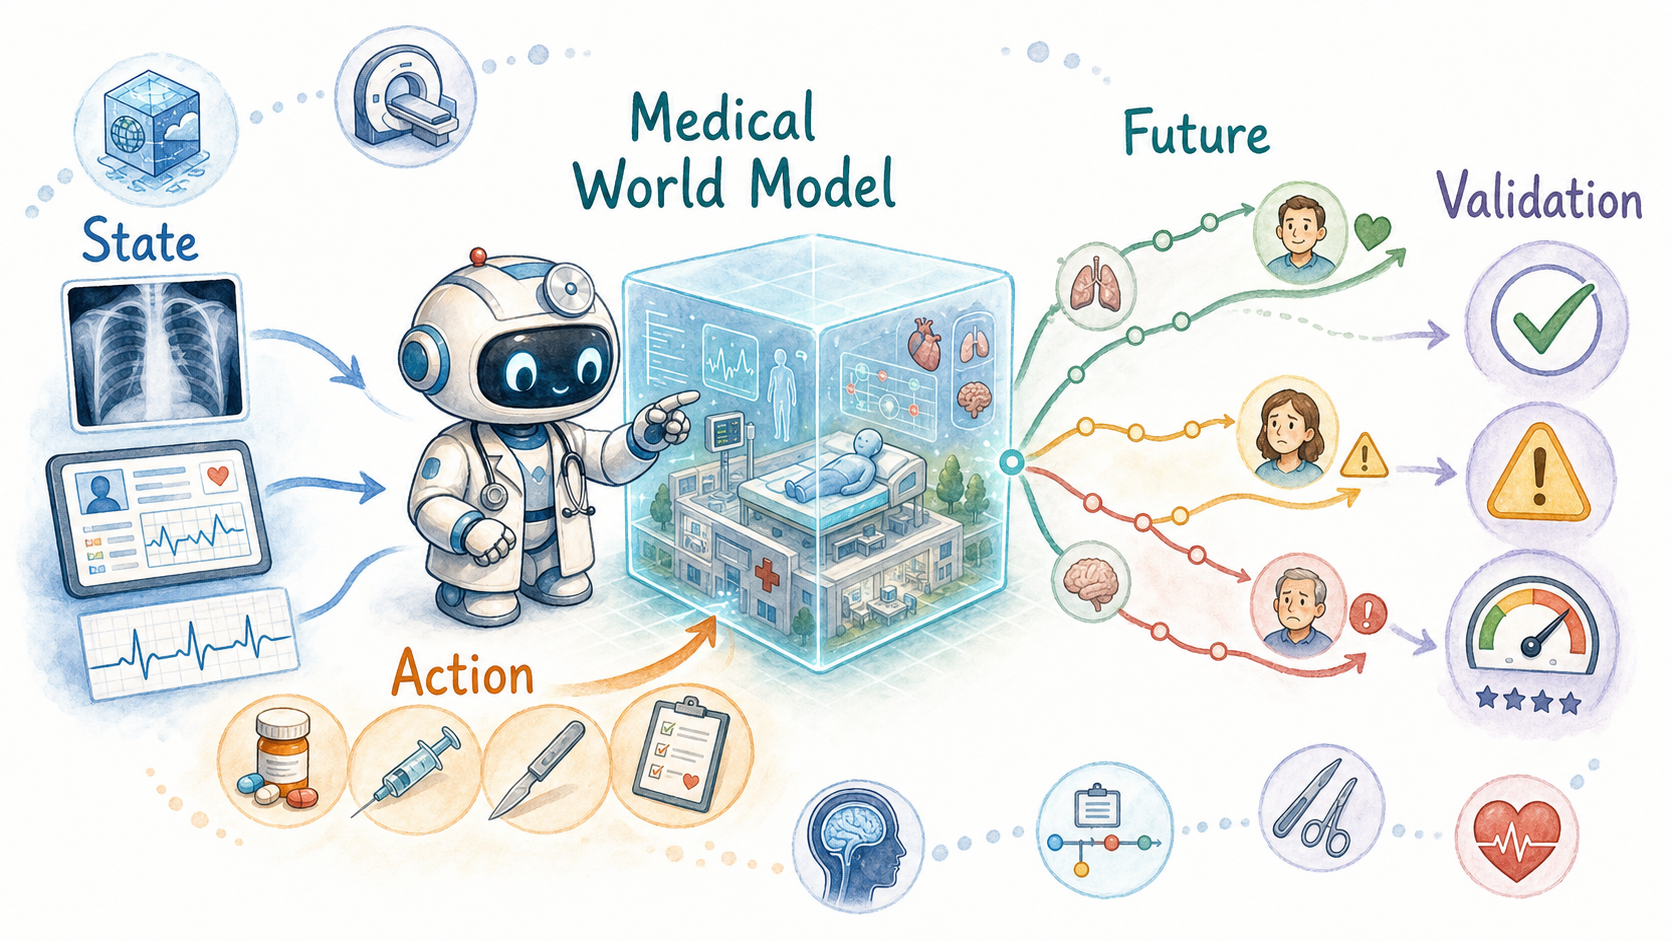
\includegraphics[width=\linewidth]{figures/fig_roadmap_imagegen_v3.png}
\caption{A visual definition of a medical world model. Patient state evidence and executable clinical actions enter a simulator-like model of the medical environment; the model rolls forward plausible future trajectories and exposes outcome or validation targets. The small visual badges indicate the paper families reviewed later in the article, including imaging, EHR trajectories, causal treatment modeling, surgical simulation, physiological signals, and general world-model backbones.}
\label{fig:roadmap}
\end{figure}


Our central standard is \emph{clinical-action validity}. A clinically meaningful state must be linked to an action that can be chosen or executed; the modeled transition must respond to that action; the resulting outcome must match the decision being invoked; and validation must address the relevant horizon and use. This standard is stricter than visual realism or trajectory plausibility. A generated future MRI can be useful for interpolation, prognosis, or education without supporting treatment selection. Conversely, an acquisition or surgical simulator may have unusually clear actions even when its patient-outcome evidence remains limited. Clinical-action validity is therefore not a binary badge. It is a way to state precisely which part of a decision claim is supported and which part is not.

Three recurrent gaps motivate this approach. The first concerns action semantics. Time, disease stage, a medication observed in the record, a desired output label, and an executable intervention play different roles, even though each may enter a model as a token or conditioning variable. The second concerns the distinction between observed and alternative outcomes. Conditioning on treatment does not by itself establish what would have happened to the same patient under another treatment. The third concerns validation. A rollout can be realistic on held-out retrospective data yet unreliable under a new policy, at a longer horizon, or for actions weakly represented in the training distribution. These gaps are not ancillary limitations; they determine the strongest defensible interpretation of a system.

The review is organized around five non-cumulative capability levels. The ordering follows the questions posed by a model, not a claim that every system should climb a single maturity ladder. Level~1 constructs a clinically meaningful state but does not model a directed future. Level~2 predicts what is likely to happen next without exposing a settable action. Level~3 simulates a future after an explicit action, while remaining agnostic about whether observational conditioning identifies a causal effect. Level~4 estimates outcomes under alternatives for the same patient or state under an explicit causal or structural contract. Level~5 uses a learned or mechanistic model to rank, optimize, or control actions. A Level~5 planner need not satisfy Level~4 counterfactual identification, and a Level~4 estimator need not implement a planner. This separation is essential in medicine, where computational capability and evidential validity frequently advance at different rates.

\paragraph{Contributions.} This survey makes four contributions. First, it provides an operational definition of medical world modeling centered on state transition and clinical-action validity. Second, it adapts prior capability ladders into five non-cumulative task contracts with explicit adjacent boundaries, giving particular attention to the transition from forecasting to action-conditioned simulation and from conditioning to counterfactual estimation. Third, it synthesizes the literature within each capability level across clinical applications and representative model designs, while using SATO-V to distinguish implemented form from evidential support. Fourth, it derives a cross-level assessment and research agenda focused on action semantics, causal identification, decision-aligned validation, external generalization, and reporting standards. The aim is not to claim ownership of the underlying progression, which has clear precedents, but to make its medical evidence boundaries useful for reading and evaluating the field.

\paragraph{Organization.} Section~\ref{sec:background} places this review relative to general world models, causal reasoning, digital twins, patient-trajectory modeling, and recent medical surveys. Section~\ref{sec:framework} defines the existence boundary, SATO-V contract, capability levels, and secondary analytical lenses. Sections~\ref{sec:level1}--\ref{sec:level5} form the core of the survey. Each begins with the minimum capability contract, examines the clinical evidence and representative designs that instantiate it, evaluates characteristic failure modes, and closes with the evidence needed to cross the next boundary. Section~\ref{sec:synthesis} then compares capabilities across applications, architectures, and SATO-V evidence without reintroducing a competing taxonomy. Section~\ref{sec:agenda} turns the recurring gaps into a research agenda and states the limitations of the review. Detailed search, coding, and boundary protocols are provided in the appendices.

\section{Scope, Genealogy, and Review Landscape}
\label{sec:background}

Medical world modeling did not emerge from a single technical lineage. The term now sits at the intersection of general world models, longitudinal clinical prediction, digital twins, causal treatment modeling, model-based decision making, and embodied medical systems. These traditions share an interest in change over time, but they disagree about what must be represented, whether actions need to be executable, and what evidence turns a plausible simulation into a clinically meaningful one. This section locates those traditions before the capability analysis. Its purpose is not to award a capability level to review or position papers, but to make clear which conceptual commitments the implemented literature inherits.

\subsection{General World Models and Model-Based Decision Making}

General world-model surveys describe a broad family rather than a single architecture. Some emphasize predictive state representations, others generative environments, and others the operational use of learned dynamics for planning or control. Surveys spanning foundation models, video generation, and autonomous driving show how easily the term expands from ``a model that predicts the world'' to ``a system that supports interaction'' \citep{Zhu2024IsSoraWorld,Ding2025UnderstandingWorldPredicting,Feng2025SurveyWorldModels}. That breadth is productive, but it also explains why terminology alone cannot organize the medical literature. A representation learner, a video generator, and a planner may all be called world models while answering different scientific questions.

Medicine makes the distinction consequential. In games or engineered simulators, the action set and transition rules are usually defined by the environment. Clinical records instead mix patient evolution with measurement, documentation, clinician behavior, access, and local practice. An accurate next-event model can therefore reproduce the care process without identifying how the patient would respond to a different intervention. The useful inheritance from general world models is not a particular backbone. It is the decomposition into state, transition, action, outcome, and model use, together with the recognition that rollout error can alter downstream decisions.

\subsection{Medical World-Model Surveys, Positions, and Definitions}

The medical-world-model literature increasingly frames the field as a progression from passive representation and forecasting toward intervention-conditioned simulation and planning. Recent reviews and perspectives describe combinations of patient state, temporal dynamics, intervention interfaces, multimodal observations, and decision support \citep{Saeed2026MedicalWorldModel,Liu2026MedicalWorldModelsReview,Feng2026StaticRiskDynamic,Wang2026TowardsBiomedicalWorldModels}. Their common contribution is to reject a purely static account of medical AI. Their definitions are not identical, however. Some include predictive state encoders within the world-model family, whereas others reserve the term for explicit dynamics or action-responsive rollout. Some treat planning as the culmination of the same ladder, whereas others distinguish simulation from policy optimization.

Adjacent clinical surveys broaden this genealogy. Computational modeling and simulation have long been evaluated as clinical tools, while clinical pharmacology and diagnostic specialties have developed their own accounts of how AI can support or distort decisions \citep{Johnson2023potentialpitfallsartificial,Walter2021Howartificialintelligence,Lesage2023Mappingusecomputational}. Virtual-brain work shows how a patient-specific computational model can connect neuroscience and clinical use without relying on contemporary world-model branding \citep{Wang2024VirtualBrainTwins}. Medical robotics and embodied-AI perspectives place the emphasis elsewhere: autonomy depends on coupling perception, interaction, human oversight, and task execution, not merely producing a realistic future frame \citep{Navab2026DyadicPartnershipDp,Liu2025ScreensScenesSurvey}. Taken together, these sources support a broad scope but also motivate a stricter operational definition. The present survey treats them as intellectual and application lineages; capability is assigned only to implemented task contracts.

\subsection{General Medical Digital Twins and Virtual Patients}

Digital twins form the largest adjacent review literature. Consensus, scoping, and broad healthcare reviews commonly describe a virtual counterpart that is linked to a physical patient or system and updated with observations over time \citep{Sun2022DigitalTwinMedicine,Cellina2023DigitalTwinsNew,Wang2023Opportunitieschallengesdigital,Vall_e2023Digitaltwinhealthcare,Sun2023Digitaltwinhealthcare,Katsoulakis2024Digitaltwinshealth}. The update relation is important: it separates an enduring twin from a one-time patient model. Yet the literature varies in how strictly this requirement is applied. Some accounts use digital twin for a patient-specific simulator, others for a predictive dashboard, and others for a broader data and decision infrastructure.

The proposed information pathways are correspondingly diverse. Reviews discuss imaging-derived anatomy, multimodal clinical data, omics, connected devices, wearables, laboratory measurements, and synthetic data as possible sources for twin construction and updating \citep{ukaniszyn2024DigitalTwinsGenerated,Papachristou2024DigitalTwinsAdvancements,Padoan2024Dynamicmirroringunveiling,Vall_e2024EnvisioningFuturePersonalized,Johnson2024DigitalTwinsHealthcare,Niarakis2024ImmuneDigitalTwins}. These sources can improve state estimation, but their presence does not establish a dynamic model. A multimodal patient representation may initialize a twin while remaining unable to forecast, simulate an action, or compare decisions.

Recent consensus and review work increasingly recognizes this distinction. Imaging, monitoring, IoT, and AI can support personalization, but a credible twin also needs a specified transition, an update rule, uncertainty, and validation tied to its intended use \citep{Iqbal2025consensusstatementon,Zhao2025Currentprogressdigital,Rudsari2025Digitaltwinshealthcare,Ooka2025EraPreemptiveMedicine,Saratkar2025Digitaltwinpersonalized,Kabir2025Digitaltwinshealthcare}. A similar issue arises at the system boundary. A twin may represent a patient, an organ, a surgical environment, a laboratory process, or a healthcare operation. These are legitimate objects, but they imply different states, actions, horizons, and outcomes.

The newest literature also connects digital twins to large language models, world models, simulation-based monitoring, assisted surgery, and complex-systems medicine \citep{Nadeem2025comprehensivereviewdigital,Sad_e2025Medicaldigitaltwins,Asciak2025Digitaltwinassisted,Domenico2025ChallengesOpportunitiesDigital,Zhou2026DigitalTwinAi,Babu2026HumanDigitalTwins}. This convergence is conceptually useful because it highlights missing components in both directions. World-model systems often lack patient-specific calibration and repeated updating; digital-twin proposals often specify a system architecture without implementing an action-sensitive transition. We therefore treat digital twin as a system-form overlay that can occur at any capability level, not as a sixth level and not as evidence of capability by name.

\subsection{Disease- and Organ-Specific Digital-Twin Literatures}

Disease-specific reviews make the value and limits of digital-twin language more concrete. Oncology work emphasizes adaptive treatment, multiscale tumor physiology, radiopharmaceutical therapy, treatment toxicity, and patient-specific response \citep{Karaman2025Fromdatadriven,John2025systematicreviewAI,Shen2025Fromvirtualreality,Omolayo2022DigitalTwinFrameworks,Thiong_o2022DigitalTwinTechnology,Rahmim2022Theranosticdigitaltwins,Wang2024Fromvirtualpatients,Witt2026DigitalTwinsCatalysts,Elsayed2026DigitalTwinModels}. These applications have clinically meaningful actions and outcomes, but they also face long horizons, treatment switching, censoring, and incomplete observation of alternative outcomes. The central challenge is consequently not whether a tumor can be rendered or parameterized, but whether the twin's response to a changed regimen is supported.

Cardiovascular twin reviews are often closer to mechanistic modeling. They connect anatomy, electrophysiology, hemodynamics, imaging, and therapy planning across atrial fibrillation and broader cardiovascular care \citep{Coorey2022healthdigitaltwin,Trayanova2023Updigitalpersonal,Thangaraj2024Cardiovascularcaredigital,Sel2024BuildingDigitalTwins,Karakasis2025DigitalTwinModels}. This structure offers interpretable state variables and intervention pathways. It also exposes parameter-identification and uncertainty problems: a model can be physiologically plausible at the population level while remaining weakly individualized for a specific patient.

Neurological, immune, musculoskeletal, and dermatological reviews illustrate still other meanings of a twin. Multiple-sclerosis and migraine work focuses on disease state and progression; immune-twin roadmaps emphasize multiscale and adaptive systems; orthopedic and arthroscopic reviews foreground geometry, mechanics, and procedural interaction; dermatology highlights observation and longitudinal monitoring \citep{Voigt2021DigitalTwinsMultiple,Gazerani2023IntelligentDigitalTwins,Laubenbacher2022Buildingdigitaltwins,Diniz2025Digitaltwinsystems,Bjelland2022TowardDigitalTwin,Akbarialiabad2024Digitaltwinsdermatology}. These literatures should not be collapsed into one application category. They are better compared by what is twinned, how it is updated, which actions are exposed, and what evidence supports the resulting prediction or decision.

\subsection{In Silico Trials, Verification, and Translation of Digital Twins}

A second digital-twin lineage is organized around evidence rather than organ system. Mechanism-based oncology, in silico trials, and AI-enabled twins raise questions about model qualification, verification, uncertainty, ethics, regulation, and implementation \citep{Wu2022Integratingmechanismbased,Strigari2025ComputationalNuclearOncology,Alharthi2025AIpoweredsilico,Samei2025FutureSilicoTrials}. These questions become more stringent as the intended use moves from explanation or training toward patient-specific treatment selection. A model may be useful for hypothesis generation without being qualified to replace a comparator arm or recommend care.

Meta-review and verification literature further shows that ``validation'' is not one operation \citep{Ringeval2025AdvancingHealthCare,Sel2025SurveyVerificationValidation,Glinkowski2026DigitalTwinsOrthopedics}. Numerical verification, biological plausibility, agreement with retrospective observations, external transportability, workflow utility, and decision impact support different claims. This observation directly motivates SATO-V: validation must be attached to the state, transition, action response, outcome, and intended decision, rather than reported as a generic property of the entire system.

\subsection{Longitudinal, Causal, and Model-Based Clinical Traditions}

Other adjacent literatures contribute pieces that digital-twin and world-model papers often leave implicit. EHR foundation-model critiques emphasize that longitudinal scale does not by itself recover patient dynamics, because records reflect coding and care processes \citep{Wornow2023shakyfoundationslarge}. Treatment-effect reviews make the identification problem explicit: individualized predictions under alternative interventions require assumptions about confounding, overlap, censoring, and temporal treatment assignment \citep{Bica2020FromRealWorld,Li2024Largepretrained}. Medical-world-model reviews that explicitly connect prediction, counterfactual reasoning, and planning help bring these concerns into the same conversation \citep{Qazi2025BeyondGenerativeAI}.

These traditions are complementary but non-interchangeable. A trajectory model can forecast the observed record without supporting intervention; a causal estimator can compare treatments without learning a general simulator; a model-based policy can optimize against learned dynamics without identifying patient-specific counterfactual effects. The survey therefore does not force them onto a cumulative maturity ladder. It asks which contract each implemented system satisfies and then evaluates the evidence needed for that contract.

\subsection{Competitive Positioning of This Survey}

Existing surveys provide valuable architecture, application, digital-twin, or capability maps. Our organizing choice is narrower: capability is the sole primary taxonomy, while paper role, clinical application, architecture, modality, and validation remain separate descriptors. Review, perspective, and conceptual papers establish genealogy and definitions but do not enter capability prevalence. General world models supply comparators but do not count as medical implementations. Digital twins are analyzed by implemented function rather than branding.

The second distinction is evidential. Papers are assigned according to the strongest implemented task contract, not the highest-level phrase in a title or discussion. SATO-V identifies where interpretation becomes uncertain: state, action, transition, outcome, or validation. This permits a constructive reading of the literature. A treatment-conditioned generator can be recognized as an action-responsive simulator without being credited with an identified treatment effect; a planner can be recognized as model-based without being treated as clinically valid. Detailed retrieval, coding, adjudication, and denominator rules are reported in Appendices~\ref{app:protocol} and~\ref{app:coding}.

Figure~\ref{fig:temporal-roadmap} provides a selective temporal view of representative lineages. It is an orientation device rather than an exhaustive chronology or a ranking.

\begin{figure}[t]
\centering
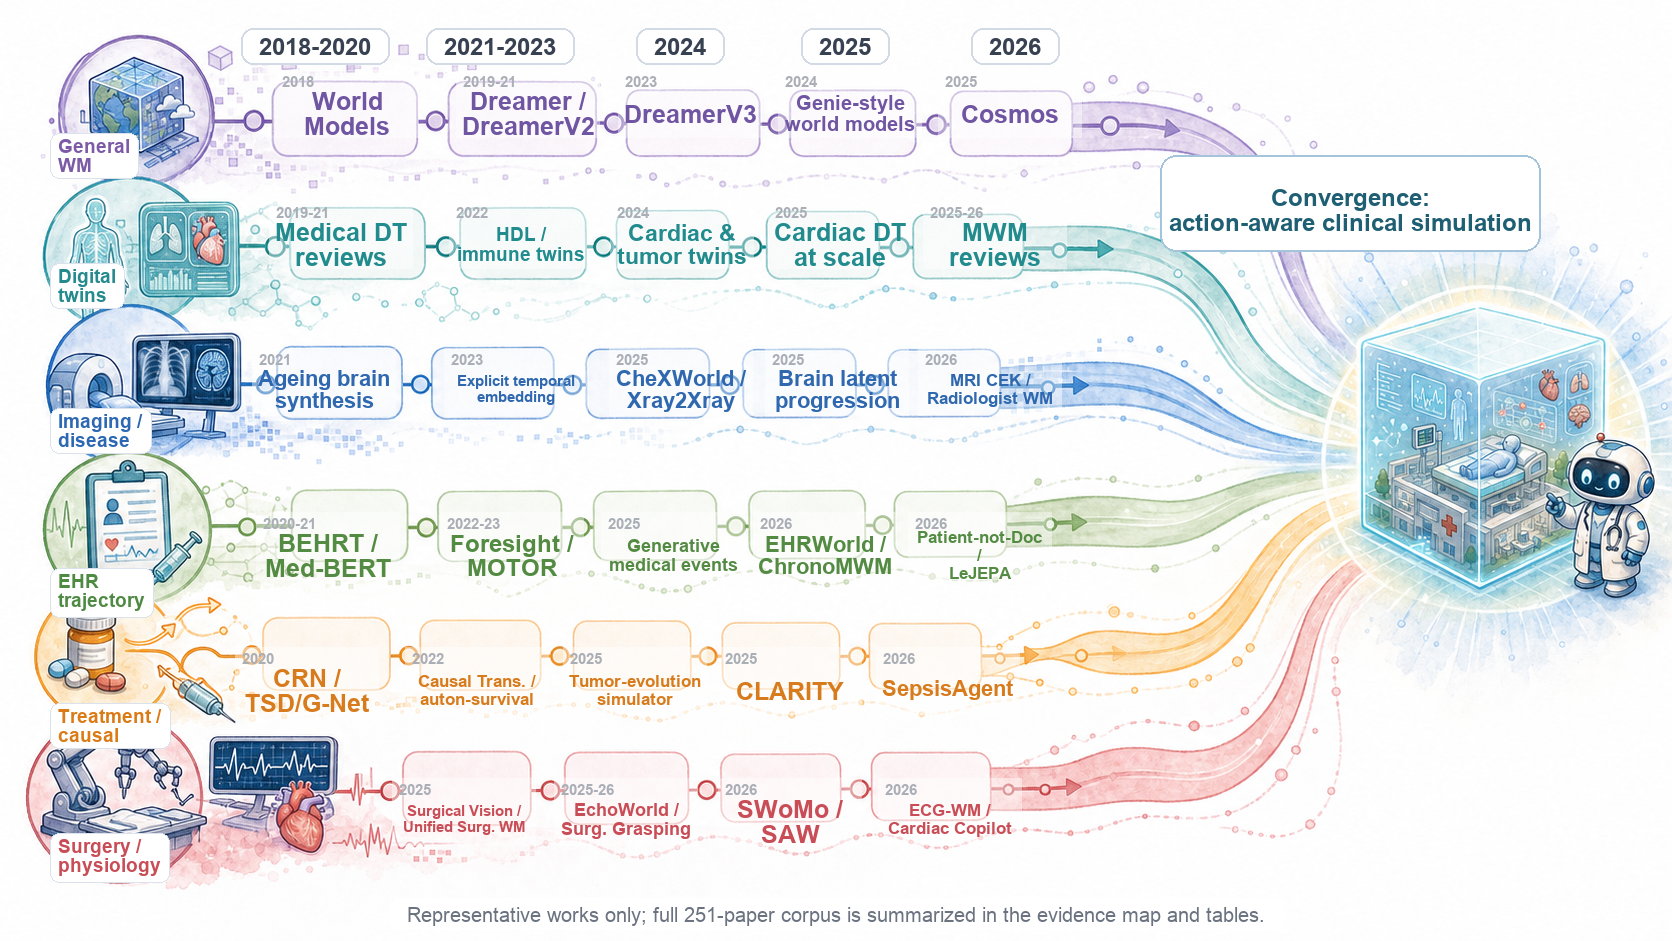
\includegraphics[width=\linewidth]{figures/fig_temporal_roadmap_imagegen_v1.png}
\caption{Temporal roadmap of representative works. Selected papers are arranged by approximate time and lineage: general world-model backbones, medical digital twins and reviews, imaging and disease-progression models, EHR trajectories, treatment and causal modeling, and surgical or physiological systems. The selection is illustrative rather than exhaustive.}
\label{fig:temporal-roadmap}
\end{figure}


\section{Foundations, Model Families, and System Building Blocks}
\label{sec:foundations}

The capability chapters focus on medical implementations. This section instead isolates the technical and conceptual building blocks that those systems borrow from general world models and adjacent decision-learning methods. The separation prevents two common distortions. General agents and driving simulators should not inflate estimates of medical capability, and a clinical policy should not be called model-based merely because it acts over time. These works are used as comparators: they clarify what state, dynamics, interaction, and planning can mean before those functions are subjected to clinical evidence requirements.

\subsection{General World Models and Latent Dynamics}

At minimum, a world model separates a represented state from a rule for changing that state. Transformer world models show that both the representation and transition can be learned as sequence prediction, with performance depending on how observations are tokenized, compressed, and rolled forward \citep{Micheli2023TransformersAreSample,Robine2023TransformerBasedWorld}. This abstraction transfers naturally to EHR events, longitudinal images, and physiological trajectories. Its medical interpretation does not transfer automatically. Tokens in a game describe an environment whose rules are defined; tokens in an EHR combine disease, observation, and clinician behavior.

The main architectural lesson is consequently functional. A latent state should retain information needed for the claimed transition and outcome; the transition should expose its temporal target and any action pathway; and the decoder or observation model should not be mistaken for the underlying dynamics. A larger latent model may improve generative fit while leaving state observability, patient identity, and action support unresolved. The later taxonomy therefore classifies the implemented contract rather than the capacity of the backbone.

\subsection{Predictive Representations and Generative Environments}

Predictive representation learning offers a route to world-model state without requiring pixel-perfect reconstruction. Joint-embedding objectives and video feature prediction learn representations by predicting missing or future latent content, while generative-environment work turns learned visual regularities into interactive sequences \citep{Assran2023Selfsupervisedlearning,Bardes2024RevisitingFeaturePrediction,Bruce2024Genie}. Hybrid use of predictive representations and diffusion priors further illustrates that representation and generation can be separate modules \citep{Park2026BeyondGenerativePriors}. These distinctions matter in medicine because a model can learn anatomically useful state while remaining below the existence boundary for a dynamic world model.

Generative realism introduces a parallel ambiguity. A model can produce a coherent frame by learning appearance statistics, but a clinical transition requires persistence of patient-specific anatomy, pathology, and physiology. Interactive generation adds another test: changing an input should alter the future through a stable action interface rather than through unconstrained prompting. These requirements motivate the Level~1/Level~2 distinction between state and directed future, and the Level~2/Level~3 distinction between temporal conditioning and executable action.

\subsection{Planning, Control, and Imagined Rollouts}

The clearest general-world-model lineage couples learned dynamics to action selection. Early latent world models and imagination-based control systems established the pattern of encoding observations, rolling latent state forward, and training or evaluating a controller inside the learned environment \citep{unknown2018WorldModels,Hafner2019DreamControlLearning,Hafner2019LearningLatentDynamics}. Dreamer variants extend this pattern across discrete and diverse domains, while MuZero demonstrates planning with a learned model that need not reconstruct every environmental detail \citep{Hafner2021MasteringAtariDiscrete,Hafner2023DreamerV3,Schrittwieser2020MuZero}. The transferable principle is that a model is decision-relevant when its predictions preserve what the planner needs, not when every observation is reproduced faithfully.

Model-predictive and hierarchical approaches place stronger emphasis on short-horizon replanning, task structure, and physical interaction. DayDreamer brings learned world models to robot learning; TD-MPC and TD-MPC2 optimize action sequences through learned latent dynamics; Director introduces hierarchical planning from pixels \citep{Wu2022DaydreamerWorldModels,Hansen2022TemporalDifferenceLearning,Hansen2024TdMpc2Scalable,Hafner2022DeepHierarchicalPlanning}. These designs offer useful engineering patterns for acquisition guidance, surgical control, and physiological management. They also reveal a medical risk: optimization searches for trajectories that exploit whatever the learned model and objective fail to constrain.

Recent systems scale the environment model itself. Diffusion-based world modeling, predictive video models, physical-AI platforms, autonomous-driving world models, and interactive real-world simulators expand visual fidelity, controllability, and domain coverage \citep{Alonso2024DiffusionWorldModeling,Assran2025VJepa2,NVIDIA2025Cosmos,Hu2023Gaia1Generative,Russell2025Gaia2Controllable,Yang2024LearningInteractiveReal}. They are useful comparators for surgical video, medical acquisition, and embodied simulation, but they remain outside the medical implementation denominator. Their actions, rewards, and safety constraints are defined for other environments. Medical transfer requires re-establishing the state, action, outcome, and validation contract rather than assuming that scale supplies clinical semantics.

\subsection{Clinical Decision Learning without an Explicit World Model}

Clinical reinforcement and imitation learning provide an important negative boundary. Policies have been learned for ventilator weaning and sepsis treatment, including approaches designed to reduce distribution-shift risk, while imitation learning has been used for surgical task execution \citep{Prasad2017ReinforcementLearningApproach,Raghu2017ContinuousStateSpace,Kaushik2022ConservativeQLearning,Kim2024SurgicalRobotTransformer}. These systems can be sequential and action-oriented without containing a world model. A value function, direct policy, or behavior-cloning transformer does not become model-based unless an explicit learned or mechanistic transition is used to evaluate, train, or optimize actions.

This boundary prevents application labels from deciding capability. ``Treatment optimization,'' ``control,'' and ``robotic autonomy'' describe intended use, not internal model use. Conversely, a medical simulator can satisfy the model component while supporting only training or offline evaluation rather than bedside control. The Level~5 contract therefore asks where the model enters the decision loop and whether removing or replacing it changes action ranking, policy learning, or control.

\subsection{Mechanistic, Causal, and Hybrid Building Blocks}

Medical world models draw on two additional traditions that are less prominent in general benchmarks. Mechanistic models specify physiological, anatomical, pharmacological, or physical structure and can expose intervention pathways directly. Causal models specify the estimand and assumptions required to compare outcomes under alternative actions. Sequence-based counterfactual estimators, G-computation networks, and causal transformers show how time-varying treatment and outcome models can be made explicit \citep{Bica2020CRN,Li2020GNet,Melnychuk2022CausalTransformer,Seedat2022TECDE}. These methods are discussed in depth at Level~4 because they implement counterfactual task contracts, even when they are not branded as world models.

Hybrid systems can combine learned representations with mechanistic state, structural constraints, or causal outcome heads. The potential advantage is not that hybrid models are valid by construction. It is that each component can carry a named responsibility: perception, state estimation, transition, intervention response, uncertainty, or planning. This modularity makes assumptions and failure modes more inspectable. It also exposes interface errors, such as a patient-specific encoder feeding population-level dynamics or a planner treating an uncertain mechanistic parameter as known.

\subsection{Cellular World Models and Biomedical Boundaries}

World-model language is also moving below the patient scale. AlphaCell, Lingshu-Cell, and GeneJEPA model cellular or transcriptomic state and, in some cases, perturbation-induced dynamics \citep{Chuai2026BuildingWorldModel,Zhang2026LingshuCellGenerative,Litman2025GenejepaPredictiveWorld}. These systems are scientifically relevant because they sharpen the same questions about state, transition, perturbation, and prediction. They are not counted as medical patient-level implementations in the primary capability distribution, since their states, actions, and validation targets operate at a different biological scale.

The boundary is analytical rather than dismissive. Cellular models may eventually supply mechanistic priors or intervention-response components for multiscale patient models. Population-health simulators may likewise inform policy without representing an individual patient. Keeping these scales visible allows the survey to discuss transfer and integration without conflating cellular perturbation, patient treatment, and health-system policy as equivalent actions.

\subsection{What Transfers to Medicine}

Across these foundations, four lessons recur. First, predictive representation is a prerequisite but not a transition. Second, a generative transition is not necessarily an action-response model. Third, action selection does not imply model-based planning. Fourth, planning through a model does not establish causal or clinical validity. These separations define the lower and upper boundaries of the five capability levels.

The medical opportunity lies in combining components that currently live in different traditions: multimodal state estimation, temporal and mechanistic dynamics, explicit interventions, counterfactual identification, uncertainty-aware planning, and decision-aligned validation. The analytical framework in the next section turns this component view into a claim-to-evidence contract.

\section{Analytical Framework}
\label{sec:framework}

\subsection{Operational Definition and Existence Boundary}

We define a medical world model as a system that represents a clinically meaningful patient or environment state and implements a directed transition over that state. The transition may be learned, mechanistic, or hybrid; it may operate in observation space, latent space, or a structured physiological state. Actions are optional for the broad existence boundary but required for the stricter action-aware levels. This definition admits future-image generators, patient-trajectory models, physiological simulators, and patient-specific mechanistic twins while excluding systems that provide only a static representation, an unconstrained generative sample, or a recommendation without an explicit model of evolving state.

Level~1 is retained because representation is the interface on which later dynamics depend and because world-model language is frequently applied to predictive encoders. We nevertheless describe such systems as world-model components unless a directed transition is implemented. This choice makes the existence boundary visible rather than allowing strong representation learning to be mistaken for rollout. A static diagnosis model, same-time modality translation system, or report generator does not become a world model merely because its backbone is predictive or generative.

The state itself can take many forms: an image or latent anatomical representation, a structured EHR vector, an event history, a waveform, organ geometry, surgical scene, physiological variable, or set of digital-twin parameters. What matters is whether the state is the object over which the transition and outcome are defined. A state that preserves texture but loses treatment-relevant anatomy may be unsuitable for intervention simulation; an EHR state that mixes patient physiology and documentation may be useful for event forecasting but ambiguous for treatment response. State quality must therefore be assessed relative to the downstream claim.

\subsection{SATO-V and Clinical-Action Validity}

SATO-V records five elements of a paper's claim. \textbf{State} identifies the modeled patient or environment state. \textbf{Action} records what can be deliberately set or executed. \textbf{Transition} specifies how state evolves and where the action enters. \textbf{Outcome} identifies the future state, endpoint, reward, or task success being predicted or optimized. \textbf{Validation} describes the evidence used to support those components. The capability level says what task form is implemented; SATO-V says how strongly the corresponding interpretation is supported. These axes must remain separate because a high-capability task can rest on weak action or validation evidence, while a lower-capability model can be rigorously validated for its narrower purpose.

Clinical-action validity is the alignment among these elements. An action should correspond to a decision or operation that can be taken: a medication, dose, regimen, surgical motion, probe movement, imaging acquisition, monitoring choice, or policy. It must be settable for the same pre-action state or history, enter the modeled transition, and lead to an evaluated post-action future. Time is not an action. Disease stage is not an action. A medication predicted as the next record event is not necessarily an action input. A desired output sketch or action-class caption is not sufficient unless it controls a meaningful transition. These distinctions prevent a generic conditioning variable from acquiring clinical semantics through wording alone.

Transitions may be implemented by diffusion or flow models, autoregressive transformers, latent state-space models, recurrent networks, graph models, neural renderers, mechanistic equations, or hybrid systems. Architecture does not determine the claim. The transition must be evaluated at the level implied by its interpretation. Pixel or token likelihood can test generative fit; biological progression requires anatomy, physiology, or outcome checks; policy use requires evidence about compounding error and the consequences of optimization. Outcomes create a parallel problem because many medical systems optimize surrogates. Image similarity, short-term stabilization, and simulated reward may be appropriate development targets, but they do not automatically support survival, safety, quality of life, or prospective workflow claims.

\begin{figure}[t]
\centering
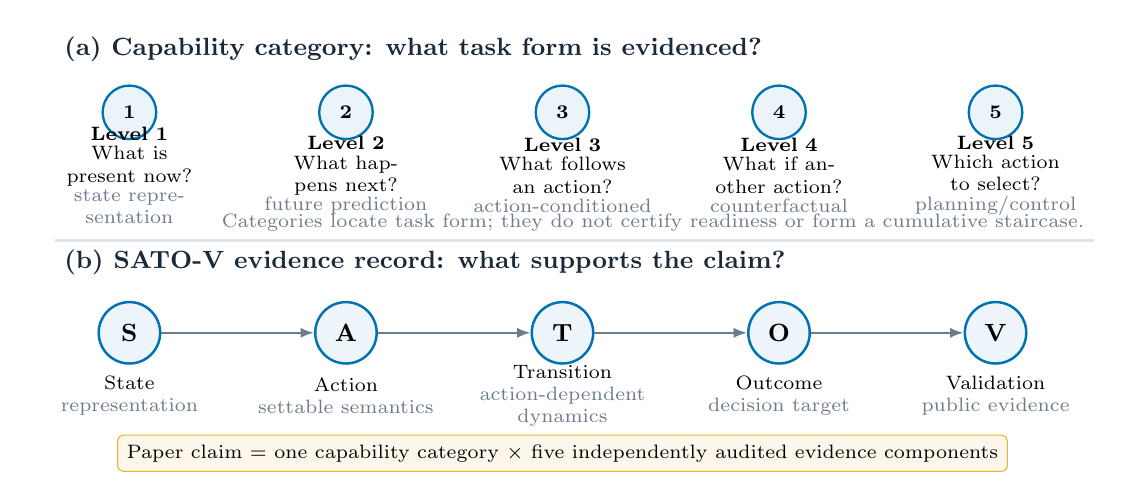
\begin{tikzpicture}[
  x=1cm,y=1cm,
  level/.style={circle,draw=mwmblue,line width=0.85pt,fill=mwmblue!8,minimum size=0.68cm,font=\bfseries\scriptsize},
  satov/.style={circle,draw=mwmblue,line width=0.9pt,fill=mwmblue!7,minimum size=0.78cm,font=\bfseries\small},
  link/.style={-{Latex[length=1.7mm]},draw=mwmgray,line width=0.75pt},
]
% Capability categories: equal columns and no connecting arrow because they are non-cumulative.
\node[anchor=west,font=\bfseries\small,text=mwmink] at (0.15,5.15) {(a) Capability category: what task form is evidenced?};
\foreach \x/\level/\question/\name in {
  1.10/1/{What is present now?}/{state representation},
  3.85/2/{What happens next?}/{future prediction},
  6.60/3/{What follows an action?}/{action-conditioned},
  9.35/4/{What if another action?}/{counterfactual},
  12.10/5/{Which action to select?}/{planning/control}}
  {
    \node[level] at (\x,4.35) {\level};
    \node[align=center,text width=2.35cm,font=\scriptsize] at (\x,3.55)
      {\textbf{Level \level}\\[-1pt]\question\\[-1pt]\textcolor{mwmgray}{\name}};
  }
\node[anchor=east,font=\scriptsize,text=mwmgray] at (13.35,2.95)
  {Categories locate task form; they do not certify readiness or form a cumulative staircase.};

\draw[mwmlight,line width=0.9pt] (0.15,2.72) -- (13.35,2.72);
\node[anchor=west,font=\bfseries\small,text=mwmink] at (0.15,2.45) {(b) SATO-V evidence record: what supports the claim?};

\node[satov] (s) at (1.10,1.55) {S};
\node[satov] (a) at (3.85,1.55) {A};
\node[satov] (t) at (6.60,1.55) {T};
\node[satov] (o) at (9.35,1.55) {O};
\node[satov] (v) at (12.10,1.55) {V};
\draw[link] (s) -- (a);
\draw[link] (a) -- (t);
\draw[link] (t) -- (o);
\draw[link] (o) -- (v);

\node[align=center,text width=2.25cm,font=\scriptsize] at (1.10,0.75) {State\\\textcolor{mwmgray}{representation}};
\node[align=center,text width=2.25cm,font=\scriptsize] at (3.85,0.75) {Action\\\textcolor{mwmgray}{settable semantics}};
\node[align=center,text width=2.25cm,font=\scriptsize] at (6.60,0.75) {Transition\\\textcolor{mwmgray}{action-dependent dynamics}};
\node[align=center,text width=2.25cm,font=\scriptsize] at (9.35,0.75) {Outcome\\\textcolor{mwmgray}{decision target}};
\node[align=center,text width=2.25cm,font=\scriptsize] at (12.10,0.75) {Validation\\\textcolor{mwmgray}{public evidence}};

\node[rounded corners=2pt,draw=mwmamber!80,fill=mwmamber!8,
      minimum width=8.2cm,minimum height=0.46cm,align=center,font=\scriptsize]
  at (6.60,0.02)
  {Paper claim = one capability category $\times$ five independently audited evidence components};
\end{tikzpicture}
\caption{The review's two analytical axes. \textbf{(a)} The non-cumulative capability levels record the implemented task form. \textbf{(b)} SATO-V records evidence for state, action, transition, outcome, and validation. A high-capability label does not imply complete SATO-V evidence.}
\label{fig:audit}
\end{figure}


\subsection{Five Non-Cumulative Capability Levels}
\label{sec:levels}

Building on recent medical-world-model rubrics \citep{Qazi2025BeyondGenerativeAI,Saeed2026MedicalWorldModel}, we use five task contracts. The categories are adapted for evidence-calibrated reading rather than presented as a new universal progression. Level~1 covers current-state representation without a directed future. Level~2 predicts a future state or event sequence without exposing a settable action. Level~3 conditions the transition on an explicit action and evaluates the resulting future. Level~4 estimates outcomes under alternative interventions for the same patient or state under an identification, structural, trial, or sensitivity contract. Level~5 uses a world model operationally to rank, select, optimize, evaluate, or control actions.

The levels are ordered for exposition but non-cumulative in meaning. Levels~2--4 relate to the movement from association to intervention and counterfactual questions \citep{Pearl2009Causality,PearlMackenzie2018BookOfWhy}; Level~5 comes from model-based decision making and reinforcement learning \citep{SuttonBarto2018Reinforcement,unknown2018WorldModels}. A planner can satisfy Level~5 by using model rollouts even when those rollouts do not identify patient-specific potential outcomes. A Level~4 causal model can estimate treatment contrasts without selecting an action. The numeric label is therefore not a clinical-readiness score. It identifies the principal question answered by the system.

The Level~2/Level~3 boundary is especially important. A model of the form $x_t=f(x_0,t)$ predicts evolution as a function of time and belongs to Level~2. A model of the form $s_{t+1}=f(s_t,a_t)$ can reach Level~3 when $a_t$ is settable, enters the transition, and changes an evaluated future. This is a task-form criterion, not a causal conclusion. Observational treatment conditioning may remain confounded by disease severity, prior response, clinician judgment, and local practice. Moving from Level~3 to Level~4 requires an explicit account of why alternative outcomes are comparable. Moving from either level to Level~5 requires operational use of the model in action selection.

\begin{table*}[t]
\caption{Capability-first reading guide. The categories identify different task contracts rather than cumulative maturity. Clinical application and model architecture describe where and how a capability is implemented; SATO-V determines whether the evidence supports the corresponding claim.}
\label{tab:capability-guide}
\centering
\small
\setlength{\tabcolsep}{4pt}
\renewcommand{\arraystretch}{1.08}
\begin{tabularx}{\textwidth}{@{}p{2.35cm}p{2.55cm}p{3.15cm}p{3.0cm}X@{}}
\toprule
\textbf{Capability} & \textbf{Clinical question} & \textbf{Minimum implemented contract} & \textbf{Typical settings} & \textbf{Common claim error or evidence bottleneck} \\
\midrule
Level 1: state representation & What is the current state? & A clinically meaningful current-state encoder, reconstruction, or same-time predictor; no directed future target. & Imaging representation, current-state phenotyping, static physiological estimation. & Treating a strong encoder or realistic generator as a rollout model. \\
Level 2: future prediction & What is likely to happen next? & A directed future state, observation, or event sequence predicted without a settable action entering the transition. & Longitudinal imaging, disease progression, EHR trajectories, physiological forecasting. & Treating time, stage, or predicted care-process tokens as interventions. \\
Level 3: action-conditioned simulation & What future follows if action $a$ is set? & A settable action enters the transition and changes an evaluated post-action state, observation, or outcome. & Treatment response, acquisition control, surgery, physiology, workflow simulation. & Reading conditioning as causal effect despite confounding or weak action semantics. \\
Level 4: counterfactual outcome reasoning & What would have happened to the same patient under another action? & Alternative-intervention outcomes with an explicit identification, structural, trial, or sensitivity contract. & Longitudinal treatment-effect estimation, survival, critical care, oncology. & Calling paired generations counterfactual without identifying the comparison. \\
Level 5: model-based planning and control & Which action or policy should be selected? & A learned or mechanistic world model is operationally used to rank, optimize, evaluate, or control actions. & Treatment planning, model-based clinical RL, surgical control, acquisition guidance. & Treating policy output, simulator success, or offline reward as clinical actionability. \\
\bottomrule
\end{tabularx}
\end{table*}


\subsection{Paper Roles, Evidence Denominators, and Boundary Cases}

The literature contains several kinds of contribution that should be visible without being treated as equivalent evidence. Implemented systems can support a capability assignment; method components establish a transition, estimator, or controller that may later be incorporated into a larger system; benchmarks and validation studies test a narrower part of the evidence chain; reviews, positions, and conceptual frameworks shape definitions and research priorities. Capability distributions in this survey are therefore based on implemented task form. The other roles remain part of the evidence map and inform interpretation, but they do not acquire a level from the capability they advocate.

Conceptual proposals illustrate why this separation is necessary. Multi-agent medical-AGI frameworks, knowledge-graph and continuous-time patient twins, cardiovascular monitoring frameworks, medical-device twins, clinical-world-model competency frameworks, and participatory chronic-care twins each identify potentially useful system components \citep{Morales2026LeJEPAIJEPA,Nye2023DigitalTwinsPatient,Iyer2025DesignanalysisTwinCardio,Riascos2022ConceptualApproachDigital,SafaviNaini2026GroundingClinicalAi,Li2026ParticipatoryDigitalTwins}. They belong in the survey because they articulate how state, interaction, updating, or human participation might be organized. They do not, however, support a high capability label until the proposed transition and decision interface are implemented and evaluated.

Negative and ambiguous cases are equally informative. Longitudinal feature fusion can improve disease classification without modeling a directed patient transition; a digital-twin label can accompany static cardiac-risk prediction; and an agentic drug-response framework can describe counterfactual behavior without providing evidence that alternative outcomes are identified \citep{Muksimova2025MultiModalFusion,Zia2025EfficientNetDigitalTwin,Baker2026ContextualInvertibleWorld}. We retain these records as boundary evidence rather than excluding them silently. Their role is to show exactly where the operational definition stops.

\subsection{Secondary Lenses: Application, Architecture, Modality, and Validation}

Clinical application answers where a capability is used. We distinguish imaging representation and acquisition, longitudinal disease progression, EHR and patient trajectories, treatment and causal modeling, digital-twin systems, and surgical, robotic, or physiological environments. These categories are intentionally secondary. Imaging systems can appear at every capability level; EHR models can range from state representation to planning; and digital twins can be conceptual, predictive, action-aware, or decision-oriented.

Architecture answers how the transition is implemented. Six broad families provide a provisional qualitative vocabulary: mechanistic or physiological models; latent state-space and recurrent dynamics; autoregressive sequence models; diffusion, flow, and video generators; graph, causal, or symbolic models; and hybrid or multimodal foundation systems. We do not report architecture prevalence before a normalized codebook has been validated. The same family can instantiate different capability levels, and an architecture described as causal does not reach Level~4 unless the estimand and supporting assumptions are explicit.

Modality, disease or organ system, and validation setting remain descriptive facets. They reveal concentration and gaps without becoming additional taxonomies. Imaging offers dense spatial observations but often weak action semantics. EHR offers long histories but entangles patient and care processes. Surgical and physiological settings expose clearer actions but impose physical and safety constraints. Validation can likewise be stronger or weaker at any level: external validation of a Level~2 forecaster may be more persuasive for its stated task than simulator-only evaluation of a Level~5 planner. Keeping these facets orthogonal allows the survey to compare what a model does, where it is used, how it is built, and how well its claim is supported without collapsing those questions into one score.

\section{Level 1: State Representation}
\label{sec:level1}

\subsection{Capability Definition and Adjacent Boundary}

Level~1 concerns the construction of a clinically meaningful current state. A model may encode an image, reconstruct a same-time observation, summarize a patient history, or infer a latent physiological state. It does not yet implement a directed transition to a future patient or environment state. This level is included because every subsequent world model depends on what is treated as the state, and because the current literature often uses world-model language for predictive representation learning. The boundary is nevertheless strict: a strong state encoder is a component of a world model, but it is not sufficient evidence that a world model exists.

The distinction is functional rather than architectural. Masked prediction, joint-embedding objectives, autoencoders, transformers, and diffusion models can all learn rich state representations. A model remains at Level~1 when its target is contemporaneous with the input or when its prediction concerns a missing region, another view, or a same-time modality rather than a directed future. A training augmentation with temporal structure does not establish a transition unless the model predicts how the represented system changes over time. This guards against equating generative complexity with dynamic capability.

The upper boundary is Level~2 future prediction. To cross it, the model must define a future target and a temporal direction. A representation that transfers well to prognosis is not itself a future model. A latent state remains a Level~1 component; when an explicit transition model uses that state to predict a future observation, the resulting system can satisfy the Level~2 criterion. This boundary matters because errors introduced at state construction propagate through every later rollout. State representation is therefore not a trivial baseline. It is the place where patient identity, anatomy, physiology, observation process, and uncertainty are either separated or entangled.

\subsection{Clinical Evidence Landscape}

Medical imaging provides the clearest examples of Level~1 state construction. Models learn anatomical or diagnostic representations from radiographs, CT, MRI, PET, ultrasound, or pathology, reconstruct missing content, translate between contemporaneous modalities, or improve image resolution. CheXWorld illustrates the representation-learning boundary, while MRI-guided PET super-resolution provides a same-time transformation without a directed future \citep{yue2025chexworld,assran2023self}. These systems can preserve clinically important structure and reduce annotation requirements, but their value at this level lies in constructing or refining a current state that later models can use, rather than in modeling how that state evolves over time.

Within imaging, representation-learning methods provide one route to such state construction. Models of radiologist reading and multimodal joint-embedding approaches learn diagnostic or anatomical representations from images and associated clinical context, while ultrasound, brain, and surgical-video JEPA variants emphasize predictive or semantic features rather than direct reconstruction \citep{li2026world,li2025self,radhachandran2026us,shah2025vision,dong2024brain,ouyang2022self}. Some of these objectives incorporate temporal, cross-view, or cross-modal structure during training. Such structure can improve the quality of the learned representation, but it does not by itself establish a directed patient-state transition at inference. The relevant distinction is therefore whether temporal information is used to construct the current state or to explicitly predict how that state changes into a future one.

Generative and reconstruction systems occupy the same Level~1 boundary through a different mechanism. MRI-to-PET synthesis, amyloid-PET super-resolution, myocardial-velocity synthesis, latent-diffusion augmentation, and patient-specific mesh reconstruction alter, complete, or refine an observation without establishing future dynamics \citep{xing2022hdl,dhinagar2024generative,shah2024enhancing,wei2020predicting,liu2026personalized}. A neighboring set of more ambiguous boundary cases arises when systems expose structured modification, controllable generation, explanation-oriented probing, or patient-specific modeling. Tumor synthesis, sketch-based editing, colonoscopy-video control, calibration-based explanations, and thoracic digital-twin frameworks illustrate such interfaces \citep{thiagarajan2022training,biller2025biophysically,kim2025tumor,huang2025interactive,fu2026depthpilot,avanzato2024lung}. These capabilities may make a system appear more simulation-like or clinically interactive, but neither controllability nor structured interrogation by itself establishes future-state modeling. Such systems remain at Level~1 when the generated, modified, or interrogated representation does not correspond to the outcome of an explicit, temporally directed transition from the current patient state.

The same state-construction boundary generalizes beyond imaging to EHRs, physiological measurements, surgical scenes, and patient-specific model initialization. An EHR encoder compresses an irregular history of diagnoses, medications, laboratory values, and procedures. A physiological model estimates a latent state from waveforms or sparse measurements. A surgical scene encoder represents anatomy, tools, and procedural phase. A digital-twin pipeline may initialize patient-specific geometry or parameters from baseline observations. Across these settings, the central scientific question is not whether a representation performs well on an arbitrary proxy task, but whether it captures the clinically relevant and transition-relevant variables required by subsequent transition and prediction components.

EHR modeling makes this distinction particularly visible. State construction can involve information extraction from clinical notes, tensor representations of longitudinal records, pretrained event embeddings, large clinical language models, multimodal virtual-patient representations, or disease-trajectory maps \citep{ying2025genie,de2018deep,rasmy2021med,yang2022gatortron,zhang2026multimodal,schulam2016disease}. These approaches differ substantially in architecture, scale, and supervision, but they share the same capability boundary: encoding a history into a representation, even when that representation transfers well to downstream prognostic tasks, does not by itself specify how the patient state evolves. Prognostic information may therefore be present in a Level~1 representation without the system having learned an explicit future transition. The use of longitudinal history as input does not change this assignment: past observations may be aggregated to estimate the current state without requiring the model to predict a future one.

The broader clinical landscape exposes a second challenge: the observed record is not necessarily equivalent to the underlying patient state. In EHR data, the record reflects decisions about what to measure, how to code observations, and when to intervene. In imaging, scanner settings and acquisition protocols can dominate a representation that appears anatomically meaningful. In surgery, camera pose, occlusion, and limited visibility can obscure the physical scene. A Level~1 model can therefore perform well on the observed data distribution while encoding nuisance structure rather than the variables that would support reliable downstream dynamics. State construction should consequently be judged not only by reconstruction or representation quality, but also by whether the resulting state is appropriate for the transition or prediction task it is intended to support.

Even once a clinically meaningful state has been individualized, a further capability boundary remains. Digital twins make this distinction especially visible: personalization or initialization of a patient state does not itself establish state-transition capability. A baseline personalized model can be clinically useful without constituting a continuously updated twin. Patient-specific geometry, parameter estimates, or risk profiles establish an individualized initial state, but they do not by themselves demonstrate how that state changes over time. At this level, digital-twin terminology is therefore treated as a system-level aspiration rather than as evidence of a specific dynamic capability. The relevant evidence is what has actually been individualized, which variables constitute the resulting state, how that state is grounded in patient observations, and, where updating is explicitly claimed, whether new observations can meaningfully revise the representation, rather than whether a broad virtual-patient architecture is described \citep{iqbal2025consensus,katsoulakis2024digital,ghatti2023digital}.

Cardiac twin initialization forms a major Level~1 evidence cluster. Inverse inference from ECG or MRI, activation-sequence personalization, electrophysiology frameworks, population-scale cardiac models, and ventricular-conduction identification all estimate patient- or organ-specific states that can later support simulation \citep{li2024toward,sanchez2025enhancing,camps2024digital,ugurlu2025cardiac,gillette2021framework,grandits2025accurate}. Related work initializes brain-perfusion twins, rare-tumor patient representations, ECG generators, and critical-care workflow twins \citep{lee2026hemopic,lammert2025large,wang2025simulator,kuruppu2025health}. Their mechanistic detail or system-level complexity can be substantial, but such complexity does not determine the capability level. Their Level~1 assignment reflects only that the available evidence does not yet demonstrate a validated, temporally directed transition from the individualized state to a future patient state.

A related state-sufficiency problem arises in small longitudinal cohorts and synthetic-patient generation. Preserving population-level distributions or multivariate trajectory statistics does not establish that an individual latent state retains the patient-specific information needed to support subsequent state-transition modeling \citep{varner2026validated}. Aggregate realism and individual state sufficiency are therefore distinct forms of evidence. A synthetic population may reproduce clinically plausible correlations or trajectories while still failing to establish that the representation of a particular patient is sufficiently informative for reliable future-state modeling. This distinction captures the general Level~1 question: not whether a representation appears realistic in aggregate, but whether it constitutes a clinically meaningful and sufficiently informative current state, with patient-specific information preserved where required by the intended downstream use.

\subsection{Representative Model Designs}

Joint-embedding and latent-prediction designs learn representations by predicting semantic or latent content rather than directly reconstructing pixels. They are attractive for imaging because they can preserve semantic structure while avoiding an emphasis on texture alone \citep{assran2023self,yue2025chexworld}. Autoencoders and multimodal encoders provide another route, particularly when a state representation must combine imaging with structured clinical variables. Diffusion models can serve at Level~1 when they reconstruct a current observation, perform same-time translation, or infer a higher-resolution image. Their placement in the hierarchy therefore depends on the prediction interface rather than on the generative architecture itself.

For EHR and physiological data, recurrent networks, transformers, and latent-variable models summarize variable-length histories. The design challenge is state sufficiency under partial observability: the latent state should retain transition-relevant information without merely memorizing the documentation process. Mechanistic models approach state construction differently by estimating interpretable parameters such as organ geometry, flow, electrophysiology, or pharmacokinetic state. Hybrid systems can use learned encoders to infer those parameters from complex observations. Such designs are particularly useful when known constraints can prevent clinically impossible latent states.

No architecture resolves state validity by itself. A compact latent variable may be efficient but difficult to inspect. A high-dimensional image state may preserve anatomy but hide causal variables. A mechanistic state may be interpretable yet miss heterogeneity that is not represented by the equations. The appropriate design depends on the transition and outcome that will follow. A survey organized by capability therefore asks what functional role an architecture plays along the path from state representation to transition modeling and future prediction, rather than assigning the architecture a fixed rank.

\subsection{Evidence Quality and Failure Modes}

Evidence at Level~1 should establish that the representation is clinically meaningful and stable for its intended use. Imaging studies can evaluate anatomical preservation, reconstruction fidelity, diagnostic consistency, and robustness across scanners or sites, as well as uncertainty calibration when uncertainty is explicitly modeled. EHR representations require patient-level splits, temporal leakage controls, missingness analysis, and transfer across coding or workflow regimes. Physiological and mechanistic state models require evaluation of parameter identifiability, sensitivity, and agreement with observed measurements. These remain tests of state validity; they do not establish the accuracy of future transitions.

The most common overclaim is to treat a strong encoder, realistic generator, or ``world-model backbone'' as evidence of rollout. A second failure is outcome leakage: a representation may encode future information through preprocessing, visit construction, or labels that would not be available at the modeled time. A third is identity loss. A model may reconstruct a plausible medical image while drifting away from the same patient's anatomy or pathology, making it unsuitable as a starting state for longitudinal simulation. A fourth is domain shortcut learning, in which site, scanner, or documentation patterns dominate clinically meaningful variation.

The appropriate next-step evidence is an explicit transition interface. Authors should state which variables constitute the state, what information is deliberately excluded, how uncertainty is represented, and which future task the state is intended to support. When a downstream transition is present, ablations should test whether the state preserves information needed across the claimed horizon. This makes Level~1 work more useful without encouraging capability claims beyond what has actually been implemented.

\subsection{Level Takeaway and Next Threshold}

Level~1 is scientifically important because state construction determines what every later simulator can know. It also marks the clearest boundary between a world-model component and a system with demonstrated predictive dynamics. The field benefits from representations that preserve patient identity, anatomy, physiology, and uncertainty, but the term ``world model'' should not obscure the absence of a directed future. At Level~1, progress is better characterized by the quality and intended role of the state than by the terminology applied to the model.

\levelsummary
{Imaging-based, EHR-based, physiological, and mechanistic models can construct clinically useful current-state representations that provide the state foundation for subsequent predictive and simulation capabilities.}
{A strong state encoder is not, by itself, a world model. Treating representation quality as evidence of rollout capability obscures the fact that a directed transition has yet to be learned or specified.}
{To reach Level~2, the system must define an explicit future target with a clear temporal direction and demonstrate prediction of that target over the stated horizon, rather than merely supporting contemporaneous reconstruction or representation transfer.}




\section{Level 2: Future Prediction}
\label{sec:level2}

\subsection{Capability Definition and Adjacent Boundary}

Level~2 predicts a future state, observation, event, or trajectory from what has already been observed. It covers longitudinal imaging, disease-progression modeling, EHR event generation, physiological forecasting, and missing-visit synthesis. Its defining question is what is likely to happen next. A model can be continuous-time, probabilistic, autoregressive, or generative and still remain at this level when no settable action enters the transition. Elapsed time, visit index, disease stage, and observed care history are covariates rather than interventions.

The lower boundary is a directed temporal target. A same-time reconstruction remains Level~1 even if its representation is predictive. The upper boundary is a settable action. To reach Level~3, the model must allow an action to be changed for the same pre-action state, use that action inside the transition, and evaluate the resulting post-action future. Predicting the medication a clinician is likely to prescribe is future prediction; simulating a patient's subsequent state after a specified medication can be action-conditioned simulation. This distinction prevents care-process forecasting from being read as intervention response.

Time-conditioned simulation is an instructive boundary. MRI CEKWorld models contrast-enhancement kinetics through $\hat I_p(t)=M_\theta(I_{p,0},t)$ \citep{Kong2026MRIContrastEnhancement}. The model has a clinically meaningful temporal transition and can generate observations at selected times. The selected coordinate is not a treatment or acquisition action, however, so the implemented claim is Level~2. It would reach Level~3 if dose, contrast agent, or acquisition policy were settable inputs whose effects on the future observation were evaluated. The distinction does not diminish the value of continuous-time modeling; it states accurately what question the model answers.

\subsection{Clinical Evidence Landscape}

\subsubsection{Longitudinal Imaging and Disease Progression}

Longitudinal imaging is a central Level~2 application because disease is often observed through repeated scans. Early work learned aging trajectories, disease states, or coupled forecasts of clinical scores and three-dimensional MRI; subsequent generative models introduced explicit temporal embeddings, sequence-aware diffusion, and conditional image synthesis \citep{Xia2021Learningsynthesiseageing,Severson2021DiscoveryParkinsons,Zhao2022Multiviewprediction,Sch_n2023ExplicitTemporalEmbedding,Yoon2023SADMSequenceaware,Dao2024ConditionalDiffusionModel}. This lineage establishes a useful distinction between cross-sectional synthesis and a patient-linked temporal target. It also exposes a recurring limitation: a model trained to match population-level change can produce a plausible future without identifying the individual mechanism that generated it.

Recent systems broaden this line from brain aging and neurodegeneration to tumor growth, pulmonary fibrosis, ophthalmology, and general four-dimensional reconstruction. Latent diffusion, flow matching, continuous-time reconstruction, and multiscale trajectory models represent irregularly sampled evolution at a selected horizon \citep{Puglisi2025BrainLatentProgression,Aghaei2025integratedpredictivemodel,Laslo2025MechanisticLearningGuided,Chen2025LearningPatientSpecific,Kapoor2025MrextrapLongitudinalAging,Zhao20254dVqGan,Disch2025CronosContinuousTime,Disch2025TemporalFlowMatching,Liu2025ImageflownetForecastingMultiscale}. A progression-map-guided model, for example, predicts patient-linked structural MRI at later follow-up in Alzheimer disease, while transition-based digital twins address sparse visits \citep{Huang2026TransitionBasedDigital,Zhao2026ForecastingAD}. Their shared contribution is temporal continuity under incomplete observation. Their shared evidentiary burden is to show that identity, pathology, and uncertainty remain credible as the forecast horizon increases.

Dynamic medical observations extend beyond conventional follow-up scans. Video and motion models synthesize endoscopy, echocardiography, ultrasound, cardiac motion, and general medical video; related systems model brain activity, ocular dynamics, inertial kinematics, and contrast-enhancement kinetics \citep{Cao2024MedicalVideoGeneration,Li2024EndoraVideoGeneration,Li2024EchopulseEcgControlled,Yu2024ExplainableControllableMotion,Caro2024BrainlmFoundationModel,Chen2025UltrasoundImageVideo,You2025TemporalDifferentialFields,Gao2026EyeworldGenerativeWorld,Delaney2026SonataHybridWorld,Kong2026MRIContrastEnhancement}. These studies make the observation process itself dynamic. ECG, motion curves, or time coordinates may control what is generated, but they do not necessarily constitute a clinical intervention. Likewise, pre-to-post-treatment image generation and latent editing can remain Level~2 when treatment is fixed by the dataset rather than exposed as a settable, validated action \citep{Yeganeh2025LatentDriftingDiffusion,Leclercq2025PrePostTreatment}.

\subsubsection{EHR Events and Patient-Trajectory Models}

EHR trajectory modeling developed from patient representations and next-event prediction toward generative foundation models of clinical timelines. Deep Patient and Doctor AI established representation learning and recurrent event forecasting; BEHRT, CEHR-BERT, Hi-BEHRT, and CLMBR then showed how temporal structure and large-scale pretraining could support downstream prediction \citep{Miotto2016DeepPatientUnsupervised,Choi2016DoctorAiPredicting,Li2020BEHRTTransformerElectronic,Pang2021CehrBertIncorporating,Li2021HiBehrtHierarchical,Steinberg2021LanguageModelsAre}. These works are important predecessors even when the learned representation is not itself a world model. They supply the state and temporal abstractions on which later generative trajectories depend.

Encoder--decoder and autoregressive systems subsequently made the future record an explicit modeling target. TransformEHR, MOTOR, Event Stream GPT, Foresight, Foresight~2, zero-shot trajectory prediction, and optimized BEHRT variants cover event sequences, time-to-event structure, and transfer across sites or tasks \citep{Yang2023TransformEHRtransformerbased,Steinberg2023MOTORTimeEvent,McDermott2023EventStreamGpt,Kraljevi_2024Foresightgenerativepretrained,Renc2024ZeroShotHealth,Odgaard2024CoreBehrtCarefully,Kraljevic2024LargeLanguageModels,Guo2024multicenterstudy}. More recent scaling studies extend this family to generative medical events, adaptive risk estimation, multi-task modeling, long-context evaluation, health-system-scale records, multimodal pathways, and recurrence-aware next-visit prediction \citep{Waxler2025GenerativeMedicalEvent,Renc2025Foundationmodelelectronic,Redekop2025Zeroshotmedical,Pang2025CEHRXGPTScalable,Kim2025MultimodalElectronicHealth,Wornow2025ContextCluesEvaluating,Rajamohan2025FoundationModelsClinical,Pellegrini2025Ehr2pathScalableModeling,Rajamohan2026ScalingRecurrenceAware}. Scale improves coverage of clinical sequences, but it does not by itself separate latent patient dynamics from documentation and care delivery.

Synthetic-EHR models form a related branch. Mixed-type longitudinal generators, diffusion models, hierarchical autoregressive systems, and semantics-guided transformers aim to preserve temporal and clinical structure while producing reusable trajectories \citep{Li2023Generatingsyntheticmixed,Kuo2023SyntheticHealthrelated,Theodorou2023SynthesizeHighDimensional,Zhou2025GeneratingClinicallyRealistic}. Delphi-2M and other large trajectory models frame this task as learning disease natural history, while digital-twin language emphasizes patient-level continuation \citep{Makarov2025Largelanguagemodels,Shmatko2025Delphi2M}. Such language should remain evidence-calibrated: generated continuity is not proof that a synthetic patient responds correctly to a changed intervention.

Two recent directions sharpen the boundary. One argues that a patient should be modeled as a changing latent system rather than as a moving document \citep{Adam2026Patientisnot}; another generates alternative patient timelines or ophthalmic trajectories \citep{Akagi2026GeneratingCounterfactualPatient,Belligoli2026OphthadtGenerativeDigital}. These are relevant to world modeling because they challenge static record prediction. Yet the word ``counterfactual'' in a title or interface does not establish Level~4: the alternative must be tied to a defined intervention and a defensible identification strategy. At Level~2, these models are best read as structured generators of possible futures.

Across this literature, outputs mix at least two dynamics: the patient's evolving condition and the healthcare system's response to it. A medication token may be generated because the model predicts clinician behavior rather than because the medication has been set as an intervention. Whether that distinction is resolved determines whether the system can be interpreted as a patient simulator.

\subsubsection{Physiological and Mechanistic Forecasting}

Physiological forecasting and digital-twin components also appear at Level~2. Graph-based patient-state forecasting, patient-specific hybrid simulation, aneurysm-flow surrogates, cardiac predictive representations, learned electrophysiology, and population virtual-patient databases each encode a temporal or mechanistic transition \citep{Barbiero2021GraphRepresentationForecasting,Sharma2025PatientSpecificDigital,Garnier2025GraphDeepLearning,Fernandes2026BeyondPatientInvariance,Zhou2026LearningCardiacElectrophysiology,Weber2026SyntheticPopulationBased}. A patient-specific autoregressive heart model similarly forecasts near-term wearable measurements \citep{Wickramasinghe2025HeartTwin}. The presence of equations, agents, or a digital-twin label does not determine the level. The relevant question is whether the audited experiment forecasts natural evolution, simulates a settable intervention, or uses the model to choose one.

These systems can support monitoring, early warning, cohort construction, and parameter estimation, but their temporal horizon and observation process must match the proposed use. Forecasting the next minute of a waveform, the next clinical event, and a five-year disease trajectory are not interchangeable forms of evidence. Mechanistic structure can improve extrapolation, yet its credibility depends on parameter identifiability and on validation against the physiological variables that the downstream decision actually uses.

\subsubsection{Surgical Video and Action-Labeled Boundary Cases}

Surgical video generation exposes this boundary directly. SurgSora, VISAGE, HieraSurg, and suturing world-model studies predict or generate procedural futures using object, hierarchy, or action annotations \citep{Chen2024SurgsoraObjectAware,Yeganeh2024VisageVideoSynthesis,Biagini2025HierasurgHierarchyAware,Turkcan2025SuturingWorldModels}. Expert assessment of zero-shot surgical video generation asks whether general video models capture clinically meaningful procedural dynamics \citep{Chen2025HowFarAre}. These studies are more informative than unconditional video synthesis, but an action label is not sufficient: the model must permit a feasible action to be changed for the same state and must validate the corresponding post-action transition before it enters Level~3.

Decision-learning comparisons also help define this boundary. DARIL, for example, contrasts imitation and reinforcement learning in surgical action planning \citep{Boels2025DarilWhenImitation}. Such work belongs in the world-model evidence map when it tests whether a predictive model contributes to action selection, but the policy result should not be attributed to a world model unless that transition model is explicit and ablated. We therefore retain these studies as boundary evidence rather than allowing planning terminology to determine their capability level.

Across applications, the common property is temporal direction without a validated, exposed decision variable. The models can support prognosis, missing-observation synthesis, trial enrichment, educational visualization, and anomaly detection. They cannot support treatment comparison merely because treatment appears somewhere in the history or because multiple futures can be sampled.

\subsection{Representative Model Designs}

Autoregressive transformers and language-model-like systems are natural for coded EHR events. They model a distribution over the next token or event sequence and can roll forward for long horizons. Their main representational challenge is to distinguish patient state from the process that records it. Recurrent networks and latent state-space models compress irregular histories and can expose an explicit latent transition. Neural ODEs and continuous-time latent models handle sparse or uneven intervals by defining evolution between observations.

Diffusion, flow, and adversarial models dominate future-image synthesis. They can preserve spatial detail and represent multimodal futures, which is valuable when disease trajectories are uncertain. Their output quality can nevertheless encourage an interpretation stronger than the training target. A visually convincing image may reflect learned population appearance rather than patient-specific biology. Mechanistic and hybrid designs provide a different bias: known equations constrain progression, while learned components estimate patient parameters or residual dynamics. These models may trade visual flexibility for interpretability and extrapolation structure.

Architecture should be selected according to the temporal question. Short-horizon observation forecasting may favor high-capacity sequence models; sparse longitudinal disease modeling may benefit from continuous-time or mechanistic constraints; image synthesis may require generative uncertainty; multimodal trajectories may require explicit alignment across measurement schedules. No family automatically resolves the action boundary. The same autoregressive or diffusion backbone can move to Level~3 only when a settable action changes the modeled future.

\subsection{Evidence Quality and Failure Modes}

Validation at Level~2 should be horizon-specific and should separate interpolation from extrapolation. One-step accuracy does not establish multi-step stability. Image studies should examine anatomy, pathology, identity preservation, and uncertainty in addition to perceptual quality. EHR studies should report patient-level temporal splits, event calibration, long-horizon degradation, missingness sensitivity, and performance under site or coding shift. Physiological models should evaluate whether errors remain acceptable at the timescale relevant to monitoring or intervention.

The most characteristic failure is to confuse prediction of the record with prediction of patient dynamics. Tests are ordered because a patient is deteriorating; medications are started in response to severity; discharge codes summarize a complex process. A model that reproduces those sequences may be useful for workflow forecasting while remaining unreliable for biological progression. A second failure is regression toward common trajectories, which can produce plausible average futures while missing rare deterioration. A third is horizon mismatch, in which a model validated at one step is discussed as a long-term simulator. A fourth is leakage through future-derived labels, preprocessing, or noncausal visit construction.

Temporal uncertainty deserves particular attention. The set of plausible futures should widen with horizon and distribution shift. Sampling diversity alone is not calibrated uncertainty, and a model can generate many images or event sequences that are all wrong in the same way. Evaluation should test coverage, calibration, and clinically important modes of failure. External cohorts with different observation and care processes are especially informative because they reveal whether the model learned patient evolution or local documentation practices.

\subsection{Level Takeaway and Next Threshold}

Level~2 is the point at which a model begins to represent dynamics rather than only state. It is already useful for prognosis and longitudinal reasoning. Its limitation is not simply the absence of a treatment input; it is that the predicted future is entangled with the policy and observation process that generated the data. Clear language about this distinction improves both the science and the clinical interpretation.

\levelsummary
{Future-image, EHR-trajectory, disease-progression, and physiological models demonstrate that clinically meaningful temporal prediction is feasible across several modalities and horizons.}
{Predicting the next clinical record does not necessarily mean predicting patient dynamics. Many apparently dynamic models learn a mixture of biology, observation, and care-process behavior.}
{To reach Level~3, a model must expose an executable action for the same pre-action state, use it in the transition, and validate a meaningful post-action future against time-only and no-action alternatives.}

\section{Level 3: Action-Conditioned Simulation}
\label{sec:level3}

\subsection{Capability Definition and Adjacent Boundary}

Level~3 models a future state, observation, or outcome after an explicit action has been set. Operationally, the model represents $p(s_{t+1},y_{t+1}\mid s_t,A_t{=}a)$, where
$A_t$ is a selectable clinical, acquisition, surgical, physiological, or management action.. This is the minimum contract for an action-aware medical world model, where the settable action enters the transition, and changes an evaluated future.

Three conditions define the boundary from Level~2. First, the action must be settable at inference for the same pre-action state or history. Second, it must enter the transition rather than serve only as a caption, classifier target, reward, or narrative prompt. Third, the system must predict a meaningful post-action future. Time, disease stage, desired output sketches, action-class text, and recorded clinician behavior do not pass the test on wording alone. Acquisition actions qualify when they control the future observation process, even if the patient state itself is unchanged. SATO-V records that narrower scope.

The upper boundary is Level~4 counterfactual outcome reasoning. Level~3 permits descriptive intervention-conditioned simulation. A treatment token may change a generated trajectory because treatment assignment is associated with disease severity and clinician behavior. Level~4 requires an explicit reason why outcomes under alternative treatments can be compared for the same patient or state. This separation allows action-conditioned systems to receive appropriate credit without importing causal language that their data and evaluation do not support.

\subsection{Clinical Evidence Landscape}

Treatment-aware imaging and disease-progression models are prominent Level~3 examples. A treatment label, treatment day, dose, or protocol variable conditions a diffusion or latent progression model that generates a post-treatment tumor or anatomical state \citep{yang2025medical,liu2019novel}. These models move beyond natural-history forecasting because an intervention enters the transition. Their clinical interpretation depends on the granularity and provenance of that intervention. A coarse label can implement the task form while remaining a proxy for patient subgroup, disease stage, or local practice.

The action-conditioned imaging cluster also includes predictive sensing in chest radiography, glioblastoma world models, multimodal physiological intervention simulation, and ontology-guided disease-risk twins \citep{yang2025xray2xray,yang2026x,wang2026brain,lutsker2026simulating,li2026modeling}. These systems expose different actions: acquisition geometry, treatment context, physiological intervention, or public-health scenario. Grouping them at Level~3 does not assert that the actions have equal clinical meaning. It records the narrower common contract that changing a settable input changes an evaluated future state or observation.

Imaging acquisition provides a observation-level action, where rotation, view selection, or probe motion changes the future measurement rather than the underlying disease process. Xray2Xray uses a selectable acquisition rotation to change the predicted radiographic observation \citep{yang2025xray2xray}. EchoWorld conditions future echocardiographic views on probe motion \citep{yue2025echoworld}. These actions are executable and directly connected to the observation process. They do not necessarily change patient biology, but they can support acquisition guidance, training, and embodied perception. This distinction shows why application and action semantics must be recorded alongside the capability level.

Surgery and robotics supply similarly explicit environmental actions. SWoMo models surgical tool-motion increments in a neuro-symbolic simulator, while surgical video world models condition future scenes on tool actions \citep{sivakumar2026swomo,rapuri2026saw,lin2024world}. The action can be instrumented, repeated, and evaluated at high temporal resolution. Their evaluation should therefore extend from visual continuity to geometry, tissue response, force, task success, and safety-relevant behavior.

The embodied cluster is broader than controllable video. Surgical vision and unified surgical world models combine scene understanding with future generation; echocardiography systems use probe motion or structural registration as the action; real-time soft-tissue simulation and long-horizon surgical modeling target physical response; large embodiment datasets support model training rather than establishing a capability by themselves \citep{koju2025surgical,unknown2025UnifiedSurgicalWorld,jiang2024cardiac,greifeneder2026autoregressive,jiang2024structure,nelson2026open,kang2026dreamreg,pan2026surgvista}. EchoWorld provides a particularly clear acquisition-action example because probe motion is explicitly coupled to the predicted view \citep{yue2025echoworld}. Across this cluster, evaluation must move from frame realism to geometry, tissue response, registration accuracy, and task-relevant safety.

EHR and physiological models occupy a more ambiguous part of Level~3. A patient simulator can qualify when a medication, dose, fluid, vasopressor setting, or management choice is deliberately supplied and the model predicts subsequent physiology. By contrast, an autoregressive model that emits the next medication or procedure as part of the record remains Level~2. Physiological priors can strengthen action semantics when interventions have known mechanisms, but retrospective treatment data still reflect selection and support limitations. Embodiment and mechanism clarify the intervention; they do not complete the causal argument.

Recent patient-trajectory and twin systems illustrate this range. EHRWorld and ChronoMedicalWorld expose longitudinal care dynamics; sepsis twins and Clin-JEPA-style patient representations connect structured history to downstream intervention modeling; cloud and standard-of-care twins place the patient model inside a broader care interface \citep{mu2026ehrworld,wang2026chronomedicalworld,lal2020development,yang2026clin,liu2019novel,bhattacharya2025soc}. The key audit question is whether an external action is supplied to the transition, not whether medications appear somewhere in the generated record.

Mechanistic and physiological twins provide more explicit state variables but still require empirical action support. Oncology twins with quantified uncertainty, stimulation-oriented virtual-brain twins, drug-aware physiological diffusion, latent physiological dynamics, and probabilistic cardiac twins all model intervention-sensitive futures at different temporal and biological scales \citep{pash2026predictive,wang2025virtual,shao2025mm,luo2026toward,giovanis2026probabilistic}. Their interpretability depends on which parameters are individualized and which intervention-response relationships are learned, assumed, or externally constrained.

Digital twins can appear at this level when they update a patient-specific state and simulate an intervention. The important distinction is implementation. A diagram of a future treatment interface is not action-conditioned evidence. A mechanistic or learned twin that accepts a defined regimen and produces a patient-specific rollout is. Patient updating, parameter uncertainty, and validation under observed interventions determine whether the twin is an operational simulator rather than an aspirational architecture.

\subsection{Representative Model Designs}

Diffusion, flow, and video generators often inject action through cross-attention, embeddings, or control channels. Their ability to model multimodal futures is attractive for treatment response and embodied scenes. The decisive design question is whether the action has a stable semantic interface and whether changing it alters outcome-relevant aspects of the rollout rather than superficial appearance. Action masking, swapping, and dose-response tests are therefore as important as image quality.

Autoregressive and recurrent patient models include actions in the event history or as separate inputs to a latent transition. Separating those roles is essential. If the model predicts an action and then feeds its own prediction back into the sequence, it may be simulating the care process. If an external action is set and the patient state is advanced conditionally, it implements the Level~3 contract. Latent state-space models can make the distinction clearer by separating observation, action, and transition variables, though identifiability and observability remain concerns.

Mechanistic, graph, and neuro-symbolic systems encode domain structure directly. Surgical simulators can impose geometry and tool constraints; physiological systems can use differential equations or known dose-response pathways; hybrid models can learn residual dynamics or patient-specific parameters. These constraints may improve extrapolation and make failures more interpretable. They can also create false confidence when parameters are weakly identified or when the mechanistic model omits clinically important heterogeneity.

The architecture should expose the action pathway. A reader should be able to identify where the action enters, what state variables it can affect, what actions are admissible, and how uncertainty propagates. An action embedding without this interface is difficult to distinguish from generic conditioning. For the same reason, architecture prevalence is less informative than whether each design makes the intervention contract inspectable.

\subsection{Evidence Quality and Failure Modes}

Level~3 validation should begin with action sensitivity. Holding the pre-action state fixed, the analysis should vary actions, compare against time-only and no-action baselines, mask or shuffle action inputs, and test whether changes occur in the expected variables and direction. Results should be stratified by common, rare, and unsupported actions. Dose-response structure, known physical constraints, and mechanistic anchors can provide additional checks. These analyses show whether action conditioning is operational; they still do not prove that the predicted difference is causal.

The characteristic overclaim is the move from ``conditioned on treatment'' to ``estimates treatment effect.'' In retrospective data, treatment choice encodes severity, biomarkers, contraindications, prior response, access, and clinician preference. A model can learn these associations and generate realistic treated trajectories while failing under a different policy. The same problem appears in surgery when action labels correlate with phase or scene, and in acquisition when a requested view can be generated without preserving three-dimensional consistency.

Other failure modes include weak action support, coarse or clinically implausible action spaces, and outcome mismatch. A model may accept actions rarely or never observed for the current state. A binary treatment label may hide dose, schedule, combination therapy, or timing. A generated image may be evaluated by perceptual similarity when the stated use requires tumor response or safety. Each limitation can coexist with a valid Level~3 task form, which is why capability and evidence quality are reported separately.

An action card would make these studies easier to assess. It should describe executability, timing, admissible range, provenance, empirical support, the state variables expected to respond, and the outcome used for validation. This information allows a descriptive simulator to be evaluated on its own terms and clarifies what further causal evidence would be needed.

\subsection{Level Takeaway and Next Threshold}

Level 3 marks the point where the modeled future becomes responsive to a selectable operation on the patient, measurement process, or clinical environment. The strongest examples arise where actions are instrumented or mechanistically defined. The main weakness arises when observational treatment labels are granted causal meaning without an identification argument. The appropriate response is not to exclude action-conditioned work, but to keep its claim at the level supported by the evidence.

\levelsummary
{Treatment, acquisition, surgical, and physiological actions can be integrated into learned or mechanistic transitions, creating useful action-responsive simulators.}
{Action conditioning is not treatment-effect estimation. In observational medicine, an explicit action input can still encode selection bias, practice patterns, and unsupported extrapolation.}
{To reach Level~4, a study must define the alternative-outcome estimand and support it through causal identification, structural assumptions, trial or quasi-experimental evidence, mechanistic constraints, or sensitivity analysis.}

\section{Level 4: Counterfactual Outcome Reasoning}
\label{sec:level4}

\subsection{Capability Definition and Adjacent Boundary}

Level~4 asks what would have happened to the same patient or state under an action other than the one observed. Formally, the target is a potential outcome or trajectory such as $P(Y_a\mid X,A{=}a')$, not merely a sampled future labeled with action $a$. The paper must state an identification, structural, trial, or sensitivity contract that explains how alternative outcomes are learned or assessed \citep{Pearl2009Causality,PearlMackenzie2018BookOfWhy}. This requirement makes Level~4 more restrictive than treatment-conditioned generation.

The lower boundary is Level~3. Sampling rollouts under two treatment tokens can reveal model sensitivity, but it does not show that their difference represents the treatment effect for the same patient. Counterfactual image editing, alternative explanations, and factual outcome prediction also remain outside Level~4 unless they estimate an unobserved clinical outcome under an alternative intervention. The upper boundary is not planning by default. A counterfactual estimator can compare interventions without choosing one, while a planner can select actions through a biased simulator without identifying counterfactual outcomes. Levels~4 and~5 answer distinct questions.

This category draws heavily from causal inference rather than from papers branded as world models. That is analytically important. The methods most explicit about potential outcomes, time-varying confounding, and treatment support often do not use world-model language, while systems described as world models frequently emphasize generation or control. The gap between these lineages is not a reason to relax the category. It identifies a missing bridge between flexible patient simulation and credible alternative-outcome estimation.

\subsection{Clinical Evidence Landscape}

The most natural Level~4 applications are longitudinal treatment-effect estimation, survival analysis, critical care, and oncology. These settings compare treatment sequences, doses, or policies over time and must address treatment-dependent censoring, competing risks, missingness, and evolving confounders. Representative methods include counterfactual recurrent networks, causal transformers, G-computation networks, and time-series deconfounding approaches \citep{Bica2020CRN,Melnychuk2022CausalTransformer,Li2020GNet,Seedat2022TECDE}. Their principal object is an alternative outcome trajectory rather than a realistic sample from the observed care distribution.

The broader treatment-effect cluster includes doubly robust representation learning, disentangled recurrent networks, heterogeneous-effect ODE discovery, and longitudinal matching through synthetic twins \citep{Zeng2020DoubleRobustRepresentation,Berrevoets2021DisentangledCounterfactualRecurrent,Kacprzyk2024OdeDiscoveryLongitudinal,Qian2021SynctwinTreatmentEffect}. Systems-based pharmacology twins add a mechanistic route to dose--response analysis \citep{Susilo2023Systemsbaseddigital}. These methods vary in representation and assumptions, but they share an explicit comparison target that is absent from descriptive action-conditioned generation.

Survival models provide a particularly clear estimand. Treatment-specific survival functions or potential-outcome regressors can compare clinically defined alternatives while accounting for censoring and treatment assignment. Open packages such as auton-survival illustrate how counterfactual estimation can be made inspectable, though software availability does not by itself guarantee identification. Oncology is a prominent application because treatment decisions and delayed outcomes are central, but the same framework applies to critical care, chronic disease, and other longitudinal interventions.

Time-varying clinical applications make the assumptions harder to avoid. Counterfactual sepsis-treatment frameworks, recurrent marginal structural networks, time-series deconfounding, G-transformers, and balanced survival models address different combinations of dynamic treatment, hidden or measured confounding, and censoring \citep{Jeter2021LearningTreatHypotensive,Lim2018ForecastingTreatmentResponses,Bica2020TimeSeriesDeconfounder,Xiong2024GTransformerCounterfactual,Chapfuwa2021EnablingCounterfactualSurvival,Nagpal2022autonsurvivalOpen}. Their outputs should be read at the level of the stated estimand and support assumptions, not as unrestricted patient-specific futures.

Medical imaging reaches Level~4 less often. A model that generates two plausible post-treatment images still faces the missing-outcome problem: only one trajectory is observed for a patient. Images can provide rich intermediate states, but they do not remove confounding or establish an outcome contrast. Mechanistic tumor or physiological models may offer structural support when their parameters and intervention pathways are validated. Their counterfactual interpretation remains bounded by model adequacy and patient-specific calibration.

Two examples show the range of possible anchors. Latent causal modeling can construct counterfactual brain MRI under an explicit structural account, while a digital-twin-guided virtual amiodarone test ties simulated intervention response to a clinically evaluated electrophysiology setting \citep{Peng2024LatentCausalModeling,Hwang2024ClinicalUsefulnessDigital}. Neither route removes the missing-potential-outcome problem. It instead makes the source of counterfactual support more visible: causal structure in one case and a calibrated mechanistic intervention pathway in the other.

The clinical evidence landscape is consequently narrower than the broader treatment-simulation literature. This scarcity should be reported as a finding rather than hidden by expansive terminology. It suggests that counterfactual capability currently resides mostly in an adjacent methodological tradition and that integration with multimodal world models remains incomplete.

This separation also changes how representative work should be selected. A treatment-conditioned generator is most informative here when it supplies an identified comparison, not simply because its outputs are visually rich. Conversely, a causal estimator belongs in the discussion even when it lacks world-model branding, because it directly addresses the alternative-outcome question that the level is meant to capture. The category is defined by the scientific estimand rather than the vocabulary of a research community.

\subsection{Representative Model Designs}

Balanced recurrent representations seek to remove information predictive of treatment assignment while preserving outcome-relevant history. Causal transformers extend this idea to long-range dependencies and time-varying treatments \citep{Bica2020CRN,Melnychuk2022CausalTransformer}. G-computation and related sequence models estimate outcomes by iterating conditional models under a specified intervention regime \citep{Li2020GNet}. Potential-outcome heads model treatment-specific outcomes directly, sometimes with propensity or weighting components. These designs make the estimand more explicit than a generic action-conditioned generator.

Graphical and structural causal models offer another route. They encode assumptions about how patient variables, treatments, measurements, and outcomes relate. Mechanistic simulators can play a similar role when biological equations specify how interventions alter dynamics. Neither structure is self-validating. Graphs require defensible causal assumptions; mechanistic systems require parameter identification and evidence that omitted processes do not dominate the decision. Hybrid models may combine flexible representation with a structured outcome or transition component, but the source of identification should remain visible.

Architecture is therefore secondary to the causal contract. A transformer described as causal does not qualify because of its name, and a small regression model can qualify when the estimand, assumptions, and validation are appropriate. The relevant design questions are which interventions are compared, over what horizon, for which population, under what support and consistency assumptions, and how time-varying confounding and censoring are handled.

\subsection{Evidence Quality and Failure Modes}

The defining validation problem is that both potential outcomes are never jointly observed for the same patient. Factual hold-out accuracy is insufficient because a model can predict observed outcomes well while estimating treatment contrasts poorly. Evidence may come from randomized or quasi-experimental variation, semi-synthetic data with known effects, trial emulation, mechanistic constraints, negative controls, held-out policy regimes, or sensitivity analyses. Each source supports a bounded claim; none turns an observational model into a universally valid patient-specific oracle.

Overlap and positivity are central. If a treatment was rarely given to patients in a particular state, the model must extrapolate to evaluate that alternative. Aggregate performance can hide this problem. Studies should report treatment support, effective sample sizes, uncertainty, and performance in weak-overlap regions. Time-varying settings also require attention to treatment-dependent censoring and post-treatment covariates. A model that conditions incorrectly on those variables can introduce bias even when its predictive metrics improve.

The common overclaim is to use the word counterfactual for any alternative generation. A clinically useful counterfactual statement must specify the estimand, intervention regime, target population, horizon, assumptions, and uncertainty. Benchmark counterfactual accuracy is valuable when the ground truth is known, but it does not automatically validate a real-patient claim. External data with different practice patterns, trial comparisons, and domain-specific sensitivity analysis can narrow that gap.

Another failure is excessive patient specificity. Population-average or subgroup treatment effects can be identified under assumptions that are insufficient for individual treatment effects. A model may output a patient-level number because its input is patient-specific, but the uncertainty in the individual contrast can remain large. Claims should match the level at which the evidence is informative.

\subsection{Level Takeaway and Next Threshold}

Level~4 is not simply a more elaborate generator. It changes the scientific target from an action-labeled future to an alternative outcome under an explicit comparison. The strongest evidence currently comes from causal sequence modeling, survival analysis, and mechanistic or semi-synthetic validation. These methods provide concepts that world-model systems need, while world models offer richer state and transition representations that causal estimators often lack.

\levelsummary
{Causal sequence, survival, structural, and mechanistic approaches provide explicit tools for estimating outcomes under alternative interventions, especially for longitudinal treatment questions.}
{Strict counterfactual evidence remains concentrated in the causal-inference lineage and is still weakly integrated with systems branded as medical world models. Generating alternatives is more common than identifying them.}
{The next threshold is not automatically Level~5. A decision system must operationally use a validated model to rank or select actions and must evaluate how transition, counterfactual, and uncertainty errors affect that choice.}

\section{Level 5: Model-Based Planning and Control}
\label{sec:level5}

\subsection{Capability Definition and Adjacent Boundary}

Level~5 uses a learned or mechanistic world model operationally to rank, select, optimize, evaluate, or control actions. The model must participate in the decision loop: it may generate candidate rollouts, provide a simulated environment, support model-predictive control or tree search, evaluate policies, or train an agent through imagined experience. A direct model-free policy and a paper that mentions planning only as future work do not meet this contract \citep{SuttonBarto2018Reinforcement}.

The adjacent boundary is functional rather than causal. Level~3 simulates a future after an action, and Level~4 estimates alternative outcomes under an identification contract. Level~5 adds operational action selection. It does not guarantee Level~4. A surgical controller can be trained in a simulator without estimating patient counterfactual outcomes. An offline sepsis planner can optimize a learned environment whose action-response estimates remain confounded. Conversely, a careful counterfactual estimator can remain at Level~4 if it never selects or ranks actions. Calling Level~5 the highest capability does not make it the strongest evidence category.

This distinction matters because optimization amplifies model weaknesses. A predictor is evaluated on states observed in the data; a planner actively searches for actions and trajectories that may exploit errors or leave empirical support. Small transition biases can compound across the horizon, and reward misspecification can direct the policy toward clinically undesirable states. Planning is thus a demanding use of a world model, not a shortcut to clinical actionability.

\subsection{Clinical Evidence Landscape}

\subsubsection{Clinical Policy Learning and Treatment Planning}

Treatment planning and model-based clinical reinforcement learning are the most direct Level~5 settings. Early sepsis work learned patient transitions for policy optimization or built explicit simulation environments, while neighboring approaches optimized treatment policies directly from observational data \citep{Raghu2018ModelBasedReinforcement,Parbhoo2018Improvingcounterfactualreasoning,Komorowski2018AIClinician,Kiani2019SepsisWorldModel}. DeepSurv and related recommenders illustrate a distinct boundary: ranking treatments from estimated outcomes is decision-relevant, but it is not automatically model-based planning over a transition system \citep{Katzman2018DeepsurvPersonalizedTreatment}. We include such studies because they reveal what a Level~5 claim must add beyond risk-adjusted treatment ranking.

Benchmarks and safety-oriented offline methods make this distinction testable. DTR-Bench supplies an in silico environment for dynamic treatment regimes, whereas inverse-constrained reinforcement learning addresses safety-critical objectives \citep{Luo2024DtrBenchSilico,Fang2024OfflineInverseConstrained}. Matching-based off-policy evaluation focuses on whether a proposed ventilation policy can be compared credibly from retrospective data \citep{Lee2025MatchingBasedOff}. These components do not all constitute medical world models, but they define the evaluation infrastructure and alternatives against which model-based planning should be judged.

Recent systems make the dynamics-to-decision connection more explicit. CLARITY, medDreamer, a general Medical World Model, and patient-dynamics agents use latent trajectories, imagined experience, or model interaction to support clinical choices \citep{Ding2025CLARITYMedicalWorld,Yang2025MedicalWorldModel2,Xu2025medDreamer,Wu2026AgentifyingPatientDynamics}. Physiology-informed intervention simulation, knowledge-guided population policy modeling, and treatment-response optimization extend this pattern across ECG, opioid-overdose policy, and clinical decision support \citep{Chen2026ECGWMPhysiology,Ma2026Policy4oodKnowledgeGuided,Qin2026TreatmentResponseOptimized}. In these systems, the model is inspectable inside the decision loop. Their claims remain bounded by retrospective support, reward design, and whether simulated action effects are reliable where the optimizer searches.

\subsubsection{Metabolic, Rehabilitation, and Public-Health Control}

Metabolic care provides one of the clearest translational pathways because glucose dynamics, sensing, and interventions can be represented at short time scales. Digital-twin-enabled precision nutrition, reinforcement-learning glycemic control, and adaptive artificial-pancreas systems span retrospective development, proof-of-concept clinical evaluation, and closed-loop control \citep{Shamanna2021Type2Diabetes,Wang2023Optimizedglycemiccontrol,Kovatchev2025InteractiveArtificialPancreas}. Their evidence is not interchangeable: a clinical outcome associated with a digital-twin program does not isolate the twin's causal contribution, whereas closed-loop control places stronger demands on calibration, fail-safes, and continual state updating.

Model-based control has also been proposed for rehabilitation and systemic inflammation \citep{Larie2022PreparingnextCOVID,Ye2025TowardsAIbased}. These settings broaden the action space from drug dosing to multimodal therapy and contextual adaptation. They also make reward validity harder. Functional recovery, inflammatory regulation, adherence, and delayed adverse outcomes cannot be reduced safely to a single short-horizon surrogate without sensitivity analysis.

\subsubsection{Mechanistic Digital Twins and Model-Predictive Control}

Mechanistic and hybrid twins can connect explicit physiology to optimization. The UVA/Padova diabetes simulator is a longstanding example of a virtual-patient environment used to develop and test control strategies \citep{Man2014UvaPadovaType}. Patient-specific optimization has also been studied for trauma surgery, radiotherapy under uncertainty, ventricular-tachycardia ablation, Alzheimer disease treatment, sepsis control, and acute-kidney-injury interventions \citep{Aubert2021DevelopmentDigitalTwins,Chaudhuri2023Predictivedigitaltwin,Chrispin2026DigitalTwinGuided,Xu2026NeuralOperatorBased,Pickard2026EhrMpcInference,Zhang2026WorldModelEnhanced}. Across these domains, the decisive evidence is not that the twin can be optimized, but that the recommended action remains stable under plausible parameter, structural, and observation uncertainty.

Level~5 is therefore not simply a synonym for reinforcement learning. Model-predictive control may use a mechanistic simulator, a learned generative patient model, or a hybrid transition and repeatedly replan as measurements arrive. Search may compare a finite set of treatment schedules without learning a policy. Both satisfy the capability contract when the model operationally ranks actions; neither establishes clinical validity without decision-level evaluation.

\subsubsection{Surgical, Acquisition, and Physiological Control}

Surgical and acquisition systems provide another route because actions are instrumented and short-horizon outcomes can be observed at high temporal resolution. World models have been used for general surgical grasping, visuomotor grasping, video-based policy learning, and open simulation for augmented dexterity \citep{Lin2024WorldModelsGeneral,unknown2025VisuomotorGraspingWorld,unknown2025SurgWorldCosmosH,Yu2024OrbitSurgicalOpen}. Related work applies goal-conditioned control to ultrasound navigation and reinforcement-learning path planning for robotic imaging \citep{Amadou2024GoalConditionedReinforcement,Bi2026AutonomousPathPlanning}. These tasks make planning technically natural, but image-space success does not demonstrate safe tissue interaction or reliable acquisition of diagnostically sufficient views.

Endovascular navigation illustrates the progression from a learned environment to a safety-constrained autonomy claim. Work on mechanical-thrombectomy navigation, online evaluation of surgical robot policies, and world-model-based endovascular intervention combines simulation, hierarchy, or policy assessment \citep{Robertshaw2025WorldModelAi,Zbinden2026CosmosSurgDVRK,Robertshaw2026SafeAutonomousRobotic,Robertshaw2026AiAutonomousNavigation}. The relevant validation extends beyond trajectory completion to collision, force, anatomical variability, recovery from error, and operator takeover. A model can support tool-motion planning or policy training in a simulator \citep{Yue2025EchoWorldLearningMotion,Rapuri2026SAWTowardSurgical}; clinical use still requires safety variables that may be absent from video realism metrics.

\subsubsection{Virtual Clinical Environments and Diagnostic Agents}

Virtual clinical environments can also train or evaluate diagnostic agents. Evolving diagnostic agents in a simulated clinic is relevant to Level~5 when the environment changes in response to tests, questions, or diagnostic actions and the agent uses those transitions to select what to do next \citep{unknown2025EvolvingDiagnosticAgents}. The key boundary is whether the environment represents a patient process or merely scores a completed answer. Diagnostic success alone does not demonstrate a world model; sequential action-dependent state change does.

Mechanistic and digital-twin systems can be optimized through model-predictive control, search, or parameterized treatment planning. Their appeal is interpretability: actions and physical or physiological constraints can be represented explicitly. Their limitation is model mismatch. A patient-specific twin built from sparse data may produce precise recommendations that are highly sensitive to uncertain parameters. Repeated state updating and uncertainty-aware planning are therefore central to the credibility of this pathway.

Level~5 also includes candidate-policy evaluation and simulator-mediated agent training when the world model is used operationally rather than as background motivation. These uses can be valuable before clinical deployment. A simulator may support rehearsal, data augmentation, stress testing, or controller pretraining even when it is not valid enough to recommend real care. The intended use determines the required fidelity: training environment, offline evaluation, and bedside decision support impose different error tolerances.

\subsection{Representative Model Designs}

Learned latent environments coupled to actor--critic algorithms or search are common model-based designs. The world model predicts latent transitions and outcomes; the planner evaluates candidate actions through imagined trajectories. Model-predictive control repeatedly replans as new observations arrive, limiting the horizon over which errors accumulate. Tree search can explore discrete interventions, while hierarchical policies can divide long clinical decisions into slower strategic and faster operational actions.

Agent systems may query a patient-dynamics model as a tool. This makes the world-model contribution visible if the agent uses simulated futures to compare actions and if ablations isolate the effect of the dynamics model. An LLM that generates a recommendation from text without an explicit transition remains outside Level~5, even when its prompt invokes a world model. Similarly, a model used only to shape reward or initialize a policy does not establish model-based planning unless it participates in action evaluation.

Mechanistic and hybrid planners use ODEs, finite-element systems, pharmacokinetic models, or rule-based environments, sometimes with learned residuals or parameter inference. They can encode hard constraints and known action pathways, which is attractive in physiology and surgery. Their decision validity depends on parameter uncertainty, structural adequacy, and how the planner behaves when observations conflict with the model. Hybrid systems should state which component supplies the state, transition, action response, reward, and uncertainty.

The planner and world model should be separable enough to inspect. Without this separation, a strong policy result cannot show whether the model learned useful dynamics, the policy exploited simulator artifacts, or the reward encoded the answer. Ablations comparing model-based and model-free variants, short- and long-horizon planning, and alternative transition models can reveal where performance originates.

\subsection{Evidence Quality and Failure Modes}

Evaluation should connect model error to decision error. In addition to predictive accuracy, studies should test compounding error across rollout depth, robustness to transition perturbations, uncertainty under unsupported actions, and sensitivity to reward or objective design. Comparisons should include clinician imitation, myopic rules, model-free baselines, and policies evaluated under the same assumptions. A planner should abstain or revert to a conservative policy when the state or action lies outside support.

Offline policy evaluation is development evidence, not prospective proof. Importance weighting, learned evaluators, or the same simulator used for training can favor the proposed policy when support is weak or model bias is shared. Semi-synthetic and mechanistic environments can provide known counterfactuals, but their validity is limited by the environment specification. External cohorts with different practice patterns, prospective silent deployment, workflow studies, and ultimately trials are needed as the intended use approaches clinical decision support.

Reward misspecification is a distinctive failure mode. Short-term physiological stabilization may conflict with mortality or recovery; image response may not align with survival or quality of life; video realism may not align with tissue safety. Optimization can exploit these mismatches more aggressively than prediction. Papers should therefore define the clinical utility represented by the reward, report alternative objectives, and examine whether the selected policy changes when surrogate assumptions are varied.

The characteristic overclaim is to treat model participation in action selection as evidence of causal or clinical validity. A Level~5 system can be computationally correct and clinically unreliable. The capability label should be paired with separate statements about intervention semantics, causal support, outcome relevance, and validation setting. This allows planning work to be recognized without equating a simulated improvement with patient benefit.

\subsection{Level Takeaway and Next Threshold}

Level~5 completes the computational decision loop, but it does not complete the clinical evidence loop. Its promise is greatest when the action space is explicit, the world model is inspectable, uncertainty constrains planning, and evaluation connects errors in simulation to errors in decisions. Its risk is greatest when optimization searches outside the support of retrospective data or exploits a surrogate outcome.

\levelsummary
{Learned, mechanistic, and hybrid world models are already used for treatment planning, policy evaluation, acquisition guidance, surgical simulation, and agent training.}
{A model participating in action selection does not establish causal or clinical validity. Planning can magnify transition bias, unsupported extrapolation, and reward misspecification.}
{The field must move beyond capability labels toward decision-level evidence: support-aware planning, calibrated abstention, external and prospective validation, and evaluation against patient-relevant outcomes.}

\section{Cross-Level Synthesis}
\label{sec:synthesis}

The five capability levels separate task form, but the field's larger patterns emerge only when those levels are crossed with clinical application, architecture, and evidence. These secondary lenses do not reclassify papers. They show where particular capabilities concentrate, which model designs recur across levels, and where SATO-V evidence most often breaks. Figure~\ref{fig:landscape} summarizes the capability--application landscape, while Table~\ref{tab:cross-level-synthesis} condenses the principal cross-level conclusion.

\begin{figure}[t]
\centering
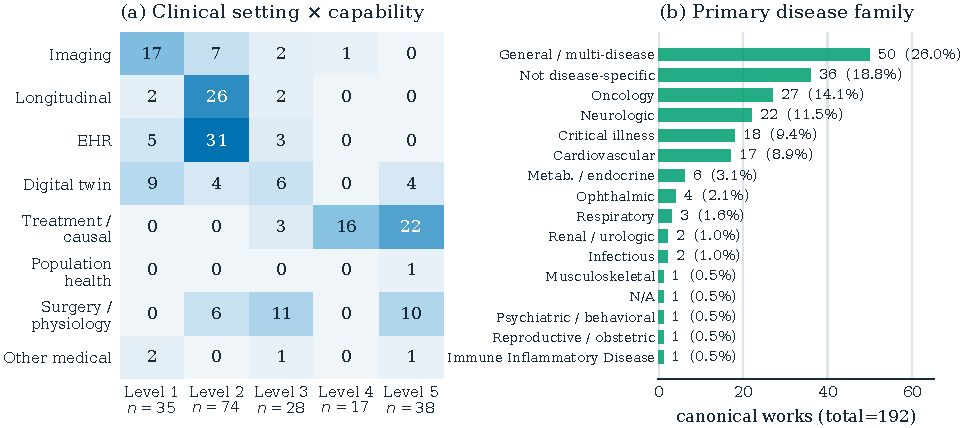
\includegraphics[width=\linewidth]{figures/fig_landscape.pdf}
\caption{Capability and clinical context. \textbf{(a)} Primary clinical application crossed with the non-cumulative Level~1--5 categories for implemented clinical canonical works with sufficient evidence for adjudication ($n{=}\MedicalImplementedTotal$). \textbf{(b)} Primary disease-family distribution for the same works. Contextual, duplicate-version, unresolved, and non-transition records are excluded.}
\label{fig:landscape}
\end{figure}


\subsection{Capability $\times$ Clinical Application}

Imaging supplies a large share of the state-representation and future-prediction literature. Its dense observations and mature generative models make Level~1 and Level~2 systems comparatively accessible. Imaging also reaches Level~3 through treatment-conditioned disease generation and acquisition control, and Level~5 through guidance or planning. The limiting evidence changes across this progression. At lower levels, patient identity and biological fidelity are central; at action-aware levels, the main question is whether conditioning represents an executable intervention; in planning, image quality must be connected to a decision-relevant endpoint.

EHR and patient-trajectory modeling spans future prediction, action-conditioned simulation, counterfactual estimation, and planning. The recurring difficulty is that state, action, and outcome can all appear as tokens in the same sequence. This makes implementation flexible but interpretation fragile. A model can forecast a medication, condition on a medication, estimate its potential outcome, or use simulated outcomes to select it. These are four different contracts. EHR models therefore benefit most from explicitly separating patient state, observation process, clinician behavior, and the intervention interface.

Longitudinal disease models bridge imaging and treatment simulation. Natural-history forecasting is Level~2; treatment-aware rollout can reach Level~3; causal comparison requires Level~4 evidence; and optimization produces a Level~5 system. Oncology and neurology are prominent because repeated imaging and clinically meaningful progression are available, but missing visits, treatment switching, censoring, and long horizons complicate validation. A visually plausible progression is not equivalent to patient-specific response.

Surgical, robotic, acquisition, and physiological systems have comparatively clear actions. Tool motion, probe movement, acquisition rotation, and controlled physiological inputs can be instrumented and repeated. This often makes the Level~2/Level~3 boundary easier to judge than in EHR. The weak point moves to physical consistency, safety, and outcome relevance. A high-fidelity training simulator may be valuable while remaining inappropriate for real-time clinical control. These applications demonstrate that clear action semantics are necessary but not sufficient for clinical-action validity.

Digital twins cut across all five levels. They can initialize a patient state, forecast natural history, simulate interventions, support counterfactual reasoning, or guide optimization. Treating the term as an independent capability would therefore hide more than it reveals. The useful questions are what is twinned, how the state is updated, which actions are exposed, what model drives the transition, and how the resulting decision is validated. A focused mechanistic twin with tested intervention response can be more informative than a broad multimodal architecture with only static prediction.

\subsection{Capability $\times$ Model Architecture}

No architecture maps to one level. Diffusion and flow models can reconstruct current observations, predict future images, or generate treatment-conditioned futures. Autoregressive transformers can forecast EHR events, emulate action-conditioned patient trajectories, or provide an environment for planning. Latent state-space models can support natural history, intervention response, and model-predictive control. Mechanistic models can serve prediction, causal simulation, or optimization depending on how actions and decisions enter. Graphical or symbolic structure reaches the counterfactual category only when it participates in a defensible identification or structural contract.

Architecture nevertheless shapes characteristic failure modes. Autoregressive systems risk reproducing documentation and clinician behavior instead of patient dynamics. Diffusion and video models risk substituting perceptual realism for biological or physical validity. Latent state-space models must address observability and uncertainty. Mechanistic systems must justify parameters, structural assumptions, and patient-specific updating. Hybrid foundation systems must state which component carries state, dynamics, intervention response, and validation. These patterns motivate a qualitative architecture lens, but not architecture prevalence claims before the codebook has been normalized.

The most promising designs are likely to combine strengths rather than select a single family. Learned representations can absorb multimodal observations; state-space structure can separate dynamics from measurement; mechanistic constraints can encode known physiology or geometry; causal components can define treatment comparisons; and planners can use uncertainty to limit action search. Hybridization is useful only when component responsibilities remain inspectable. A large multimodal system that obscures the action pathway is harder to validate than a narrower model with a clear contract.

\subsection{Capability $\times$ SATO-V Evidence Quality}

State is generally the strongest SATO-V component. Imaging, EHR, waveform, and surgical-scene representations are often well specified. Action and validation are weaker. At Level~2, the central issue is whether forecast accuracy reflects the patient or the record-generating process. At Level~3, the action may be explicit while its empirical support and causal meaning remain uncertain. At Level~4, the missing potential outcome forces reliance on assumptions, trials, quasi-experiments, mechanistic constraints, or semi-synthetic anchors. At Level~5, model and reward error are amplified by optimization, while evaluation is often retrospective or simulator-based.

Outcome validity cuts across the ladder. A future image, event token, physiological state, or simulated reward may be an appropriate technical target. The claim becomes miscalibrated when that target is treated as a patient-centered outcome without a validated link. Validation should therefore be decision-aligned rather than uniformly ``stronger'' at higher levels. A Level~1 state model may require external representation transfer; a Level~2 forecaster requires horizon-specific calibration; a Level~3 simulator requires action-sensitivity and support tests; a Level~4 estimator requires identification and sensitivity evidence; and a Level~5 planner requires policy-level and prospective evaluation.

\subsection{What the Field Has Actually Achieved}

The field has clearly moved beyond static prediction. Future-state modeling is established across imaging, EHR, and physiology, and action-conditioned simulation is visible in treatment, acquisition, and embodied settings. Model-based planning is also implemented in several clinical and simulator-mediated systems. The evidence is less complete than the capability labels suggest. Counterfactual identification remains concentrated in adjacent causal methods, and prospective decision-level validation remains uncommon relative to the clinical ambition of the work.

The principal gap is therefore not a missing generative backbone. It is the integration of four elements that are currently distributed across different literatures: rich patient state, executable action, credible alternative-outcome reasoning, and decision-aligned validation. Imaging and foundation models contribute representation and generation; causal methods contribute estimands and assumptions; mechanistic twins contribute structural constraints; model-based control contributes operational decision loops. A clinically credible medical world model will need these elements to meet in one inspectable evidence chain.

\begin{table*}[t]
\caption{Cross-level evidence synthesis. Capability identifies the implemented task form; the remaining columns summarize what the reviewed literature supports and what must change before a stronger clinical interpretation is justified.}
\label{tab:cross-level-synthesis}
\centering
\small
\setlength{\tabcolsep}{4pt}
\renewcommand{\arraystretch}{1.08}
\begin{tabularx}{\textwidth}{@{}p{2.6cm}p{4.0cm}p{4.0cm}X@{}}
\toprule
\textbf{Level} & \textbf{Observed achievement} & \textbf{Main evidence gap} & \textbf{Next threshold} \\
\midrule
Level 1: state representation & Clinically useful image, EHR, physiological, and mechanistic state construction. & No directed transition; representation may encode nuisance or observation-process structure. & A calibrated future target supported by a stable, uncertainty-aware state. \\
Level 2: future prediction & Longitudinal images, patient events, disease states, and physiological trajectories can be forecast. & Record prediction is often conflated with patient dynamics; long-horizon and external calibration are limited. & An executable action that enters the transition and changes an evaluated future. \\
Level 3: action-conditioned simulation & Treatment, acquisition, surgical, and physiological actions can control simulated futures. & Conditioning may reproduce selection bias or superficial action correlations rather than intervention response. & An explicit alternative-outcome estimand with identification or structural support. \\
Level 4: counterfactual reasoning & Causal sequence, survival, and mechanistic methods estimate outcomes under alternative interventions. & Both potential outcomes are unobserved; support, confounding, and individual-level uncertainty remain difficult. & Operational use of a validated model in action ranking or selection, with decision-error analysis. \\
Level 5: planning and control & World models support treatment planning, policy evaluation, acquisition guidance, and simulator-mediated control. & Optimization amplifies transition bias, unsupported actions, and reward misspecification; prospective evidence is sparse. & Support-aware planning, calibrated abstention, external validation, and patient-relevant prospective evaluation. \\
\bottomrule
\end{tabularx}
\end{table*}


\section{Research Agenda and Limitations}
\label{sec:agenda}

\subsection{Action Semantics and Causal Identification}

The first priority is to define actions before modeling their effects. Medical datasets contain treatment orders, administrations, dose changes, procedures, monitoring choices, clinician recommendations, and workflow events. These variables differ in executability, timing, adherence, and causal meaning. Future work should report the action set, admissible range, decision time, provenance, and empirical support, and should distinguish an observed care event from an action that can be set in simulation. This simple discipline would resolve many Level~2/Level~3 boundary disputes and expose when a proposed intervention lies outside the data.

Action-aware simulation should also be paired with negative controls. Holding state fixed while varying treatment, masking action inputs, comparing with time-only models, and testing known dose-response or physical relationships can reveal whether the model uses the intervention as intended. These tests do not establish causality, but they prevent action tokens from serving as decorative conditioning. In EHR systems, separating the patient transition from the clinician or observation policy is especially important. Joint models can be appropriate, but the modeled process should be named.

The next step is to connect flexible world models with causal identification. Counterfactual sequence models, trial emulation, instrumental or quasi-experimental designs, mechanistic constraints, and sensitivity analyses should not remain peripheral to medical-world-model development. A productive integration would retain rich multimodal state and generative uncertainty while making the estimand, support assumptions, censoring, and time-varying confounding explicit. The aim is not to force every simulator to claim treatment effects. It is to make clear when such a claim is intended and what evidence it requires.

\subsection{Decision-Aligned Evaluation, Uncertainty, and External Validation}

Evaluation should follow the decision horizon. One-step image or event prediction may be sufficient for interpolation but not for long-range planning. A treatment simulator should be evaluated on action sensitivity and clinically relevant response, not only perceptual quality. A planner should be assessed on how transition error changes selected actions, not only on simulator reward. Each capability level therefore needs a distinct evaluation contract rather than a shared leaderboard.

Uncertainty must constrain use. Generative diversity is not enough; systems should estimate when state, action, or horizon lies outside support. Calibration, coverage, conformal or ensemble methods, model disagreement, and mechanistic sensitivity can all contribute, but the output should affect the decision loop. A planner that recognizes uncertainty yet still optimizes aggressively outside the training distribution has not solved the problem. Abstention, conservative fallback policies, and uncertainty-aware action constraints should be evaluated explicitly.

External validation is particularly important because clinical dynamics are shaped by population, site, scanner, coding, workflow, and treatment policy. A model trained at one institution may fail because the patient distribution changes or because the observation and care processes differ. External cohorts should therefore report which component shifted. For action-aware systems, differences in treatment practice can be informative rather than merely inconvenient: they test whether the model learned patient response or local policy. Prospective silent deployment and workflow studies can provide an intermediate step between retrospective evaluation and interventional trials.

The capability-specific requirements above are summarized as a validation ladder in Appendix~\ref{app:coding}. Its rungs are evidence types rather than a universal score: the appropriate evidence depends on the intended use, and one rung does not substitute for causal identification or action support at another.

\subsection{Data Coverage, Generalization, and Hybrid Mechanistic Models}

Current work concentrates in settings with repeated measurements, large archives, or simulatable environments. Rare diseases, multimorbidity, long-term outcomes, underrepresented populations, and cross-system trajectories remain less visible. Scaling the same architecture on more records will not automatically solve this gap because actions and outcomes are often sparsely observed. Data collection should be organized around decisions and longitudinal follow-up, with explicit documentation of treatment timing, adherence, censoring, and missingness.

Multimodal integration should be selective. Imaging, EHR, genomics, physiology, pathology, behavior, and environment can all contribute to patient state, but broad fusion is useful only when each modality supports the transition or outcome being modeled. A narrow, validated simulator can be more scientifically informative than a universal patient representation whose action pathway is unclear. Missing-modality behavior and asynchronous measurement should be treated as part of the model rather than hidden by imputation.

Hybrid mechanistic models are a promising response to sparse interventions and distribution shift. Known anatomy, conservation laws, dose-response relationships, pharmacokinetics, tissue mechanics, and safety constraints can restrict implausible rollouts. Learned components can estimate residual dynamics, infer patient parameters, or process complex observations. The key challenge is calibration: structural assumptions and parameter uncertainty must be reported, and the model should be tested where learned and mechanistic components disagree. Hybrid does not mean valid by construction.

\subsection{Benchmarks and Reporting Standards}

Benchmarks should be stratified by capability rather than mixing static prediction, natural-history forecasting, action-conditioned simulation, counterfactual estimation, and planning. For Level~2, tasks should distinguish interpolation, one-step prediction, and long-horizon rollout. For Level~3, they should define executable actions, hold pre-action state fixed, and include no-action and action-shuffle controls. For Level~4, they should state the estimand and provide trial, quasi-experimental, semi-synthetic, or mechanistic anchors with overlap and sensitivity analyses. For Level~5, they should evaluate policy robustness, reward sensitivity, support violations, and the relationship between model error and decision error.

A compact reporting card can make claims comparable without prescribing one model family. It should state the modeled state and time scale; action variables, timing, and provenance; transition mechanism; outcome and clinical horizon; uncertainty; data and action support; validation setting; and intended use. Authors should identify the capability level they implement and separately state whether causal or clinical validity has been evaluated. Reviewers can then judge a narrow claim on its own evidence rather than rewarding the most ambitious vocabulary.

Adjacent evidence records clarify what a benchmark cannot establish. A multicenter longitudinal cohort can characterize prognostic trajectories and outcome associations without providing ground truth for an intervention simulator \citep{Li2021TrajectoriesPerioperativeSerum}. Conversely, a digital-twin framework can optimize secure data management without implementing patient-state dynamics \citep{Alotaibi2026CostOptimizedTwin}. Such studies remain relevant to data provenance and evaluation design, but they should not be counted as capability implementations. Reporting the paper role alongside the benchmark task prevents infrastructure, cohort evidence, and simulated dynamics from being conflated.

Open code and data improve auditability but should not be treated as proxies for scientific quality. Clinical data may be restricted for legitimate reasons. When data cannot be released, cohort construction, event vocabularies, preprocessing, censoring, splits, and evaluation protocols become more important. Paper-linked code, model weights, synthetic examples, and executable evaluation scripts can still support reproducibility. Resource status should be timestamped because repositories and releases change.

\subsection{Review Limitations}

This survey is an ML-facing capability and evidence review, not a disease-specific clinical systematic review, regulatory assessment, formal risk-of-bias analysis, or meta-analysis. Terminology creates retrieval bias: papers using ``world model'' are easier to find than methods with equivalent task contracts under different names. We mitigate this by including adjacent digital-twin, trajectory, causal, and model-based decision literatures, but the boundary cannot be exhaustive.

The capability taxonomy is adapted from prior medical-world-model frameworks, and its categories remain analytical choices rather than a settled community standard \citep{Qazi2025BeyondGenerativeAI,Saeed2026MedicalWorldModel,Liu2026MedicalWorldModelsReview,Wang2026TowardsBiomedicalWorldModels}. The non-cumulative interpretation, clinical-action boundary, and SATO-V evidence contract are designed to make those choices explicit. Some papers remain reasonable boundary cases, particularly when actions are partially implemented or causal assumptions are implicit. The detailed coding protocol preserves uncertainty rather than forcing every study into an overprecise label.

The literature is also moving quickly. Preprints, publication status, repositories, and validation evidence can change. The corpus therefore supports a current evidence synthesis rather than a final census of the field. Architecture is discussed qualitatively because a normalized codebook has not yet been validated across the full literature; no prevalence claim is made from free-text descriptions. Finally, public evidence may understate private implementation or clinical testing. Throughout the review, ``not publicly evidenced'' should not be read as proof of absence.

These limitations do not remove the main conclusion. They reinforce the need to separate task capability from evidential strength and to make boundary judgments inspectable. Formal submission should be preceded by author-level verification of every included record, refreshed metadata and resources, and domain review of the strongest clinical claims.

\section{Conclusion}
\label{sec:conclusion}

Medical world modeling is not a single architecture or application. It is a set of claims about representing state, predicting change, responding to action, comparing alternatives, and using simulated futures to choose decisions. A capability-first structure makes these claims comparable, while SATO-V shows where their evidence is strong or incomplete. The resulting picture is neither that the field is limited to static prediction nor that clinical planning has been solved. Future prediction and action-conditioned simulation are now visible across imaging, EHR, disease progression, physiology, and embodied environments; credible counterfactual reasoning and decision-level validation remain much less integrated with these systems.

The central research task is therefore not generation alone. It is to align a clinically meaningful state with an executable action, an action-sensitive transition, a decision-relevant outcome, and validation appropriate to the intended horizon. This alignment gives lower-level work a precise and useful role, prevents planning language from substituting for evidence, and defines concrete thresholds for progress toward clinically credible world models.


\bibliography{references}
\bibliographystyle{tmlr}

\appendix
\section{Search and Study-Selection Protocol}
\label{app:protocol}

The evidence map was designed as an ML-oriented review rather than a PRISMA-style review of clinical interventions. Retrieval combined structured searches of scholarly indexes and publisher metadata with citation expansion from papers that used terms including ``medical world model'', ``clinical world model'', ``patient world model'', ``digital twin'', ``patient trajectory'', ``treatment planning'', ``counterfactual'', and ``simulation''. The broad boundary included papers that self-identified as world models, near-core work on longitudinal patient trajectories, patient-specific digital twins, treatment-aware disease simulation, surgical and physiological simulators, model-based clinical decision making, and foundational general-domain work needed to interpret the methodological lineage.

Ordinary static diagnosis or prognosis studies were excluded unless they directly informed the representation boundary. Preprints and published versions were linked by persistent identifier, normalized title, and version provenance so that one canonical work contributed at most once to quantitative summaries. Contextual reviews, perspectives, and general-domain anchors were retained for interpretation but were not combined with implemented clinical systems in application-specific denominators.

The selection strategy is intentionally broader than the operational definition. Broad retrieval makes terminology drift visible; the capability and existence rules prevent that breadth from being interpreted as evidence that every retrieved paper implements a world model. Records without sufficient full-text evidence for capability adjudication were retained as unresolved but excluded from primary capability and application distributions.

\subsection{Screening Boundary}

Core papers explicitly identify as medical or clinical world models or directly implement state-transition simulation in a clinical domain. Near-core papers include EHR trajectory models, patient-specific digital twins, treatment-aware progression models, causal longitudinal outcome models, model-based clinical decision systems, and surgical or physiological simulators. Background papers are included only when they define concepts used to interpret the core literature. A static predictor can appear as boundary evidence but is not counted as an implemented transition model unless a directed future is present.

\begin{table}[t]
\caption{Positioning against adjacent reviews and surveys. Prior work supplies the clinical and methodological context; this review adds non-cumulative capability boundaries and an orthogonal evidence analysis.}
\label{tab:review-positioning}
\centering
\small
\begin{tabularx}{\linewidth}{@{}p{0.28\linewidth}p{0.26\linewidth}X@{}}
\toprule
\textbf{Literature} & \textbf{Primary organizing axis} & \textbf{What this review adds} \\
\midrule
Medical and biomedical world-model position/review articles \citep{Qazi2025BeyondGenerativeAI,Saeed2026MedicalWorldModel,Liu2026MedicalWorldModelsReview,Wang2026TowardsBiomedicalWorldModels} & Capability ladders; coupled state, dynamics, and intervention roadmaps; and multiscale biomedical roles from data engines to planning substrates & A non-cumulative boundary contract plus corpus-wide adjudication of implemented capability, clinical facets, uncertainty, and public evidence. \\
Digital-twin surveys and consensus work \citep{Iqbal2025consensusstatementon,Katsoulakis2024Digitaltwinshealth,Ghatti2023DigitalTwinsHealthcare} & Patient-specific virtual counterparts, mechanistic modeling, and clinical ambition & A learned-model capability scale that prevents digital-twin language from implying individualized rollout or validated action response before those are evidenced. \\
Structured-EHR foundation-model reviews \citep{Guo2026Systematicreviewfoundation} & EHR pretraining, trajectory modeling, and clinical event prediction & A state--action distinction that separates predicting care-process tokens from simulating patient response under settable interventions. \\
This review & Capability scale $\times$ SATO-V evidence contract, with application and architecture as secondary lenses & Paper-level claim calibration that separates implemented capability from action validity, causal support, clinical setting, and validation strength. \\
\bottomrule
\end{tabularx}
\end{table}


\section{Evidence Coding, Adjudication, and Uncertainty}
\label{app:coding}

For each study, coding records the modeled object, temporal target, action semantics, transition mechanism, outcome, counterfactual support, planning role, and highest reported validation setting. The clinical facets include primary application, disease family, organ system, modality, and evaluated task. Public code, model, and data status are recorded separately from scientific capability because availability can change and does not establish validity.

A capability decision follows two stages. The existence gate first asks whether a clinically meaningful state and directed transition are implemented. The level decision then identifies the strongest task contract supported by the method and evaluation. Level~1 denotes state representation without directed transition; Level~2 denotes future prediction without a settable action; Level~3 requires a settable action that enters the transition and changes an evaluated future; Level~4 requires an explicit alternative-outcome identification or structural contract; and Level~5 requires operational use of a world model in action ranking, optimization, evaluation, or control. Ambiguity is retained in confidence and boundary notes rather than resolved from titles or self-description alone.

The review distinguishes unavailable evidence from negative evidence. A component is coded as not publicly evidenced when the paper and linked official artifacts do not describe it clearly enough to inspect. This designation does not imply that the component is absent from private implementation. Quantitative summaries include only canonical works with sufficient evidence for a capability decision; contextual and unresolved records are reported separately.

The manuscript uses Level~1--5 consistently. Legacy database values are transformed only at the display layer, so the naming change does not alter source records or quantitative results.

\begin{table}[t]
\caption{Capability distribution among implemented canonical works with sufficient evidence for adjudication ($n{=}217$). Each work is counted once; contextual, duplicate-version, unresolved, and non-transition records are excluded. Levels are non-cumulative: Level~5 does not certify Level~4.}
\label{tab:levels}
\centering
\small
\setlength{\tabcolsep}{4pt}
\renewcommand{\arraystretch}{1.08}
\begin{tabularx}{\linewidth}{@{}>{\raggedright\arraybackslash}p{2.55cm}Xrr@{}}
\toprule
\textbf{Capability category} & \textbf{Operational decision rule} & \textbf{$n$} & \textbf{\%} \\
\midrule
Level 1: current-state modeling & Current-state representation, calibration, or same-time synthesis; no directed future target. & 38 & 17.5 \\
Level 2: future prediction & Directed future state or observation without a settable action entering the transition. & 74 & 34.1 \\
Level 3: action-conditioned simulation & A settable action changes an evaluated, meaningful post-action future. & 35 & 16.1 \\
Level 4: counterfactual outcome reasoning & Alternative-intervention outcomes are estimated with an explicit causal identification contract. & 17 & 7.8 \\
Level 5: planning/control & A world model is operationally used to rank, select, optimize, or control actions or policies. & 53 & 24.4 \\
\bottomrule
\end{tabularx}
\end{table}

\begin{table}[t]
\caption{Primary clinical-application distribution among implemented clinical works with sufficient evidence for adjudication ($n{=}192$). Each canonical work is counted once. General-domain anchors and non-clinical biomedical context papers are excluded from this denominator.}
\label{tab:tracks}
\centering
\small
\setlength{\tabcolsep}{6pt}
\renewcommand{\arraystretch}{1.08}
\begin{tabularx}{\linewidth}{@{}Xrr@{}}
\toprule
\textbf{Primary clinical application} & \textbf{$n$} & \textbf{\%} \\
\midrule
Counterfactuals and treatment planning & 41 & 21.4 \\
EHR and patient trajectories & 39 & 20.3 \\
Longitudinal disease progression & 30 & 15.6 \\
Medical imaging representation & 27 & 14.1 \\
Surgical, robotic, and physiology models & 27 & 14.1 \\
Patient and health-system digital twins & 23 & 12.0 \\
Other medical settings & 4 & 2.1 \\
Population-health policy simulation & 1 & 0.5 \\
\midrule
\textbf{Total} & \textbf{192} & \textbf{100.0} \\
\bottomrule
\end{tabularx}
\end{table}

\begin{table}[t]
\caption{Validation ladder for medical world-model claims. The rungs are evidence types rather than a score: the required rung depends on the intended use, and evidence at one rung does not substitute for causal identification or action support at another.}
\label{tab:validation-pyramid}
\centering
\small
\setlength{\tabcolsep}{4pt}
\renewcommand{\arraystretch}{1.08}
\begin{tabularx}{\linewidth}{@{}p{2.35cm}p{3.35cm}Xp{3.25cm}@{}}
\toprule
\textbf{Evidence rung} & \textbf{What it can establish} & \textbf{Minimum useful evidence} & \textbf{Typical overclaim} \\
\midrule
Internal retrospective & Performance on held-out observations from the same data regime. & Patient-level splits, leakage controls, horizon-specific error, and relevant static baselines. & Generation quality is treated as decision validity. \\
External or multicenter & Robustness to site, scanner, coding, workflow, or population shift. & Prespecified external cohorts and subgroup-specific failure reporting. & One external mean score is treated as universal transportability. \\
Expert or clinician review & Clinical coherence and recognizable failure modes. & Blinded, task-specific ratings with agreement and explicit rejection criteria. & Plausibility substitutes for outcome or causal evidence. \\
Counterfactual or policy & Behavior under alternative actions within stated assumptions and support. & Explicit estimand, overlap diagnostics, sensitivity analysis, and trial-, simulator-, or semi-synthetic anchors. & Benchmark counterfactual accuracy is treated as patient-level truth. \\
Prospective workflow or trial & Effect on a real process, decision, or patient-relevant endpoint. & Registered protocol, monitoring, predefined endpoints, and appropriate comparator. & Retrospective gains are assumed to transfer to deployment. \\
\bottomrule
\end{tabularx}
\end{table}


\section{Detailed Boundary Cases and Reviewer Checklist}
\label{app:boundaries}

\subsection{Boundary Cases}

\paragraph{Time conditioning versus action conditioning.} MRI CEKWorld predicts contrast-enhancement appearance at a selected elapsed time \citep{Kong2026MRIContrastEnhancement}. The model implements a directed temporal transition and is therefore Level~2. Time is not an executable intervention, so the system does not reach Level~3 unless a contrast dose, agent, or acquisition action is exposed and validated.

\paragraph{Care-process prediction versus patient simulation.} Foresight and related EHR generators predict longitudinal clinical events \citep{Kraljevi_2024Foresightgenerativepretrained,Waxler2025GenerativeMedicalEvent}. A medication or procedure emitted as the next event remains part of the predicted record. The model reaches Level~3 only when an external action can be set for the same history and the subsequent patient state is evaluated.

\paragraph{Treatment conditioning versus treatment effect.} Treatment-aware tumor and longitudinal imaging models can reach Level~3 when treatment changes the generated future \citep{Yang2025MedicalWorldModel,Liu2025TreatmentawareDiffusion}. They reach Level~4 only when the comparison between alternatives is supported by an explicit estimand and identification, structural, trial, or sensitivity argument.

\paragraph{Planning versus clinical actionability.} CLARITY, patient-dynamics agents, and model-based sepsis RL operationally use simulated trajectories for decisions and therefore exemplify Level~5 capability \citep{Ding2025CLARITYMedicalWorld,Wu2026AgentifyingPatientDynamics,Raghu2018ModelBasedReinforcement}. The label does not establish that the simulated action response is causal, that the reward is patient-centered, or that the policy is ready for clinical use.

\paragraph{Embodied action versus outcome validity.} Surgical tool motion, probe movement, and acquisition rotation provide clear executable actions \citep{Sivakumar2026SWoMoNeuroSymbolic,Yue2025EchoWorldLearningMotion,Yang2025Xray2XrayWorldModel}. They satisfy the Level~3 task-form boundary when they alter the modeled future, but visual or control success does not substitute for physical safety or clinical outcome validation.

\subsection{Checklist for Authors and Reviewers}

\begin{enumerate}[leftmargin=*]
\item \textbf{State:} What patient or environment state is represented, at what time scale, and which clinically important variables may be missing?
\item \textbf{Action:} Can the input be deliberately set for the same pre-action state? Is it an executable intervention, acquisition, or control, or only time, context, or an observed care event?
\item \textbf{Transition:} Where does the action enter, what variables can it affect, and is the model learned, mechanistic, or hybrid?
\item \textbf{Outcome:} Is the target a future observation, surrogate, treatment response, control success, or patient-relevant endpoint? Does it match the stated use?
\item \textbf{Validation:} Are horizon, support, uncertainty, external shift, causal assumptions, and decision consequences evaluated at the level required by the claim?
\item \textbf{Capability language:} Does the manuscript distinguish representation, future prediction, action-conditioned simulation, counterfactual reasoning, and planning rather than using them interchangeably?
\end{enumerate}

\begin{table*}[t]
\caption{Representative boundary cases spanning the existence gate and Level~1--5. Outside-scope examples are retained because branding or optimization language alone does not establish a patient or environment transition.}
\label{tab:core-matrix}
\centering
\scriptsize
\setlength{\tabcolsep}{3.0pt}
\renewcommand{\arraystretch}{1.05}
\begin{tabularx}{\textwidth}{@{}p{3.1cm}cp{2.4cm}p{3.6cm}Xp{1.1cm}@{}}
\toprule
\textbf{Paper} & \textbf{Level} & \textbf{Setting} & \textbf{Action contract} & \textbf{Transition contract} & \textbf{Code} \\
\midrule
CheXWorld: Exploring Image World Modeling for Radiograph Representation ... & 1 & medical imaging & Mask locations and image/domain transformation parameters are training conditions, ... & JEPA-style latent prediction across spatial context and image transformations; no future ... & \cgood yes \\
Enhancing Amyloid PET Quantification: MRI-Guided Super-Resolution Using Latent ... & 1 & medical imaging & No settable clinical action enters the model. & An MRI-guided latent diffusion model reconstructs a higher-resolution PET image for ... & \cgood yes \\
MRI Contrast Enhancement Kinetics World Model & 2 & medical imaging & Elapsed time is a query coordinate; contrast dose, agent, ... & A conditional generative model predicts contrast-enhanced MRI at arbitrary future time ... & \cgood yes \\
Forecasting individualized progression of Alzheimer's disease using structural ... & 2 & longitudinal progression & No treatment, acquisition, or clinical action is supplied; target ... & A progress-map-guided GAN generates the same subject's MRI at one- and ... & \cgap no* \\
SWoMo: Neuro-Symbolic World Model for Cataract Surgery Simulation & 3 & surgery/robotics & Explicit surgical tool-motion increments control tip position, orientation, articulation, ... & A rule-based Godot simulator advances geometry and tool-tissue interactions; a conditioned ... & \cgood yes \\
Treatment-aware Diffusion Probabilistic Model for Longitudinal MRI Generation ... & 3 & longitudinal progression & A target future treatment type and day are supplied; ... & Treatment-day embeddings condition a diffusion and segmentation network to generate the ... & \cgap no* \\
auton-survival: an Open-Source Package for Regression, Counterfactual Estimation, ... & 4 & treatment/causal & A treatment arm or exposure is supplied for counterfactual ... & The package fits treatment-specific survival functions and counterfactual survival regressors, with ... & \cgood yes \\
Double Robust Representation Learning for Counterfactual Prediction & 4 & treatment/causal & A binary treatment assignment indexes the two potential-outcome heads. & Double-robust representation learning combines treatment-specific outcome models with entropy-balancing weights that ... & \cgood yes \\
Agentifying Patient Dynamics within LLMs through Interacting with ... & 5 & treatment/causal & A settable 5-by-5 grid of intravenous-fluid and vasopressor-dose combinations. & A learned GRU clinical world model predicts the next physiological state ... & \cgood yes \\
ECG-WM: A Physiology-Informed ECG World Model for Clinical ... & 5 & treatment/causal & Drug identity, dose, and protocol drawn from a clinically ... & ODE-regularized latent diffusion simulates post-intervention ECG trajectories conditioned on drug action. & \cgap no* \\
LeJEPA + I-JEPA: A World-Model-Grounded Multi-Agent Framework for ... & outside & medical imaging & Prompt rewriting and report constraints are orchestration operations, not ... & No learned future-state transition is implemented; the released notebook labels LeJEPA ... & \cgood yes \\
A cost-optimized medical digital twin framework for secure ... & outside & other medical & ILP, PATI-Greedy, and HybridQeGA assign each computing task to ... & No learned or mechanistic patient, workflow, or infrastructure state transition is ... & \cgap no* \\
\bottomrule
\end{tabularx}
\vspace{2pt}
\\{\scriptsize Code: {\color{mwmteal}\faCheck} paper-linked public artifact; {\color{mwmamber}\faAdjust} partial/related artifact; {\color{mwmgray}\faMinus} no verified public study code or not applicable.}
\end{table*}


\section{Database Fields and Corpus Summary}
\label{app:database}

The evidence database records bibliographic identifiers and version relations; inclusion role; primary and secondary clinical applications; capability level; modality; disease and organ system; clinical task; state representation; action or intervention; transition model; outcome or reward; counterfactual and planning support; datasets and access conditions; code and model availability; validation setting; source locations; confidence; and adjudication status. Architecture remains a provisional field in this draft. Quantitative architecture analysis will be added only after a stratified coding study establishes stable definitions and resolves disagreements across model families.

The corpus summary tables are descriptive rather than measures of clinical maturity. Capability counts report implemented task form. Application counts describe the primary clinical setting. Resource counts describe what was publicly verifiable at the time of review. None of these dimensions substitutes for causal validity, external transportability, prospective evaluation, or regulatory readiness.

\ifworkingdraft
\paragraph{Living resource.} A maintained reading list is available at \url{https://github.com/lanqz7766/awesome-medical-world-models}.
\fi

\begin{table*}[p]
\caption{Representative works across six clinical applications. Capability, application, disease family, modality, task, and public resource status are independent fields; digital twin is treated as a system-form overlay.}
\label{tab:track-works}
\centering
\scriptsize
\setlength{\tabcolsep}{3pt}
\renewcommand{\arraystretch}{1.02}
\begin{tabularx}{\textwidth}{@{}p{3.45cm}ccp{2.45cm}p{1.9cm}Xp{1.1cm}@{}}
\toprule
\textbf{Representative work} & \textbf{Year} & \textbf{Level} & \textbf{Disease family} & \textbf{Modality} & \textbf{Evaluated task} & \textbf{Code} \\
\midrule
\multicolumn{7}{@{}l}{\textit{Medical imaging}} \\
CheXWorld: Exploring Image World Modeling for Radiograph Representation ... & 2025 & 1 & general or multidisease & radiograph & representation & \cgood yes \\
Xray2Xray: World Model from Chest X-rays with Volumetric ... & 2025 & 3 & general or multidisease & radiograph & action conditioned simulation & \cgap no* \\
MRI Contrast Enhancement Kinetics World Model & 2026 & 2 & oncology & MRI & future observation synthesis & \cgood yes \\
\addlinespace
\multicolumn{7}{@{}l}{\textit{Longitudinal progression}} \\
Forecasting individualized progression of Alzheimer's disease using structural ... & 2026 & 2 & neurologic disease & MRI & future observation synthesis & \cgap no* \\
Treatment-aware Diffusion Probabilistic Model for Longitudinal MRI Generation ... & 2025 & 3 & oncology & MRI & treatment conditioned simulation & \cgap no* \\
Explicit Temporal Embedding in Deep Generative Latent Models ... & 2023 & 2 & oncology & CT & future observation synthesis & \cgood yes \\
\addlinespace
\multicolumn{7}{@{}l}{\textit{EHR trajectories}} \\
EHRWorld: A Patient-Centric Medical World Model for Long-Horizon ... & 2026 & 3 & general or multidisease & EHR & future forecasting & \cgap no* \\
ChronoMedicalWorld: A Medical World Model for Learning Patient ... & 2026 & 3 & renal urologic disease & EHR & disease progression & \cgap no* \\
The Patient is not a Moving Document: A ... & 2026 & 2 & oncology & EHR & future forecasting & \cgap no* \\
\addlinespace
\multicolumn{7}{@{}l}{\textit{Digital twins}} \\
A Framework for the generation of digital twins ... & 2021 & 1 & not disease specific & MRI & representation & \cgap no* \\
Development of Digital Twins to Optimize Trauma Surgery ... & 2021 & 5 & musculoskeletal disease & CT & planning decision support & \cgap no* \\
A Novel Cloud-Based Framework for the Elderly Healthcare ... & 2019 & 3 & general or multidisease & wearable sensor & operations resource simulation & \cgap no* \\
\addlinespace
\multicolumn{7}{@{}l}{\textit{Treatment and causal modeling}} \\
ECG-WM: A Physiology-Informed ECG World Model for Clinical ... & 2026 & 5 & cardiovascular disease & physiology & planning decision support & \cgap no* \\
Learning to Treat Hypotensive Episodes in Sepsis Patients ... & 2021 & 4 & critical illness & EHR & treatment policy learning & \cgap no* \\
auton-survival: an Open-Source Package for Regression, Counterfactual Estimation, ... & 2022 & 4 & oncology & demographics clinical attributes & treatment response & \cgood yes \\
\addlinespace
\multicolumn{7}{@{}l}{\textit{Surgery, robotics, and physiology}} \\
SWoMo: Neuro-Symbolic World Model for Cataract Surgery Simulation & 2026 & 3 & ophthalmic disease & surgical video/robot & simulation training & \cgood yes \\
EchoWorld: Learning Motion-Aware World Models for Echocardiography Probe ... & 2025 & 3 & not disease specific & US/echo & acquisition guidance & \cgood yes \\
SAW: Toward a Surgical Action World Model via ... & 2026 & 3 & not disease specific & surgical video/robot & simulation training & \cgap no* \\
\addlinespace
\bottomrule
\end{tabularx}
\end{table*}

\begin{table}[t]
\caption{Public-resource status at the review date. Code categories describe publicly verifiable artifacts; ``not found'' does not imply that private code is absent. Unresolved full texts are excluded from the primary scientific distributions.}
\label{tab:openness}
\centering
\small
\begin{tabular}{p{1.7cm}p{7.0cm}r}
\toprule
\textbf{Axis} & \textbf{Category} & \textbf{Count} \\
\midrule
Code & paper-linked public code verified & 111 \\
Code & public but partial/related or without weights & 6 \\
Code & claimed, announced, by request, or pending & 19 \\
Code & not found, unavailable, proprietary, or unreleased & 96 \\
Code & not applicable to review/perspective & 68 \\
Full text & sufficient evidence for paper-level review & 300 \\
Full text & unresolved and excluded from primary distributions & 23 \\
\bottomrule
\end{tabular}
\end{table}



\end{document}
